\documentclass[12pt, xelatex,ja=standard,jafont=hiragino]{bxjsarticle}

\usepackage{phyexp3}
\usepackage{natbib}
\usepackage{graphicx}
\usepackage{amsmath}
\usepackage{listings}
\usepackage{url}
\renewcommand{\lstlistingname}{リスト}
\lstset{
  basicstyle={\ttfamily},
  identifierstyle={\small},
  commentstyle={\smallitshape},
  keywordstyle={\small\bfseries},
  ndkeywordstyle={\small},
  stringstyle={\small\ttfamily},
  frame={tb},
  breaklines=true,
  columns=[l]{fullflexible},
  numbers=left,
  xrightmargin=0em,
  xleftmargin=3em,
  numberstyle={\scriptsize},
  stepnumber=1,
  numbersep=1em,
  lineskip=-0.5ex
}
\usepackage[
 xetex,
 setpagesize=false,%
 bookmarks=true,%
 bookmarksdepth=tocdepth,%
 bookmarksnumbered=true,%
 colorlinks=true,%
 linkcolor=black,
 pdftitle={},%
 pdfsubject={},%
 pdfauthor={},%
 pdfkeywords={}%
]{hyperref}
\CJKspace

\newif\ifdraft
\draftfalse
%----
\year{2026} %実施年度
\supervisor{野間 春生、高橋 治輝、中村 文彦} % 担当教員


\author{長谷川　瑛二} % 氏名を記述してください
\authorid{26002403098} % 学籍番号
\mailaddr{is0791pi@ed.ritsumei.ac.jp} % メールアドレス
\class{D1} % クラス（D1, D2）


%グループの情報（共同作業者名）
\groupid{4} % グループ番号
\projectname{SPACE SORT} % 作品タイトル
\director{篠田　知幸} % ディレクタ

\programmera{池内　飛翔} % プログラマ1
\programmerb{矢口　健} % プログラマ2 いない場合は空欄{}にする
\programmerc{} % プログラマ3 いない場合は空欄{}にする
\programmerd{} % プログラマ4 いない場合は空欄{}にする

\modelera{長谷川　瑛二} % モデラ1
\modelerb{} % モデラ2 いない場合は空欄{}にする
\modelerc{} % モデラ3 いない場合は空欄{}にする
\modelerd{} % モデラ4 いない場合は空欄{}にする

%\drafttrue % 提出時には行の先頭に% をつけて%\drafttrueとしてください

\finalchecktrue
%----本文はここから---

\begin{document}
\maketitle

\section{実験を受講するにあたっての自分の目的と課題}
\ifdraft
\href{https://scrapbox.io/phyexp3/VR実験の進め方}{実験の資料}
に記載した本実験全体の目的・課題を自分で解釈し、この実験を通して、自分で得たい知識と経験を``自分の目的''として設定し、その目的を達成するための課題を、``自分の言葉''で述べる。なおテキストのコピペと見られる場合は減点の対象とする。
\fi
% 以下に本文を書く
本実験を受講するにあたっての私の目的は，VR課題作品の制作を通じてVRのメディア処理とそれを描画するためのシミュレーション技術，並びにインターフェース技術について理解し習得することである．VR機器は多様なセンサを搭載しており，それを物理エンジンであるUnityで活用するという技術の組み合わせを学ぶことによって，コンピュータ上の情報世界と現実世界を繋ぐ技術の構築を学ぶ．また本実験は４人グループの共同であるため，チームとして１つの作品を完成させる共同開発の方法を学ぶことができる．これまでにソフトウェアのチーム開発は未経験であるため，円滑にコミュニケーションを取りながらプロジェクトを進めるための方法を模索しつつ習得することを目的とする．



\section{物理シミュレーションの実装}
\ifdraft
章の冒頭で、なにを対象として物理シミュレーションするのかについて説明する。
\href{https://scrapbox.io/files/661f545b621c8200257a6a94.pdf?title=VR実験別冊テキスト.pdf}{VR実験別冊テキスト}を参考にして、物理シミュレーションの対象について、パラメータを含めて工学的に説明することが求められる。必要に応じて図を効果的に用いる。

この冒頭部分は2.1節、2.2節に共通する部分になる。すなわち、今回の実験では同じ物理現象を複数の方法を用いて実装し、それを比較するのであるから、それらで重複する部分はここに書いておく。
\fi
% 以下に本文を書く
本章における物理シミュレーションは，球体を空中から落下させる自由落下運動を調査対象としている．JavaScriptのライブラリの一つであるThree.jsを用いたWebブラウザ上でのシミュレーションと，物理エンジンであるUnity上でのシミュレーションを比較し，この二つの環境の違いを理解する．またそれぞれの解析結果を理論値と比較することによって実環境とシミュレーション環境との差を考える．ここで両環境での物理条件を示す．初期状態において，直径1$m$である球体は床面から20$m$の高さで静止しており，シミュレーションの開始と共に自由落下を始める．また球体と床面との間の反発係数は0.8としており，重力加速度は9.8$m/s^2$である．本実験では球体は床面に対して垂直に衝突するものとし，空気抵抗の影響を考慮しないものとする．

\subsection{JavaScriptでの物理シミュレーションの記述方法と実装結果}
\ifdraft
2.1節では球の落下と衝突のシミュレーションの数学的な計算方法と、JavaScriptでの実装の方法について、数式や図表、コードの一部を交えて説明する。また、結果のCGのスクリーンショット、さらに、球の落下を示すシミュレーションの結果を時系列のグラフで示し、その特徴を論述する。

記述方法は、レポートを読んだ第三者が理解し、それを実装することができる十分な情報が含まれている（再現できる）必要がある。たとえばソースコードが提供されている場合はそのソースコードの参照方法などを含む必要がある。

レポートに用いるグラフ等は、工学的に正しいグラフであることが求められる。線のタイプ、軸のラベル、凡例、単位などに留意すること。また、十分に高い解像度である必要がある。グラフを画面に表示し、そのスクリーンショットをそのまま使う解像度の低い図面や、画面をカメラで撮影したようなものは認められない。グラフはラスター形式（jpg, pngなど）の画像ファイルの場合、十分に高い解像度（150dpi以上）とすること。おすすめはPostScriptやSVG, PDFなどのベクター形式としてグラフを出力することである。
\fi
% 以下に本文を書く
2.1節ではJavaScriptを用いた球体の落下と衝突のシミュレーションについて，その実装方法を数学的，物理学的な視点を交えて解説する．またその結果について実際のスクリーンショットや時系列データをグラフで示すことによってその特徴を論ずる．

まずはJavaScript上での球体落下のシミュレーションの実装方法について解説する．大部分のコードは講義用に配布されたものであり，その一部分を改変した．改変したのはボールが衝突した時の速度の再計算部分である．反発直後の物体の速度は，面に対して垂直に衝突した場合-1倍となり，かつ元の速度の反発系数倍となる．このことからこの速度の再計算に関するコードは，RoEを反発係数として

\begin{equation}
    ball_velocity.y = -1 * ball_velocity.y * RoE;
\end{equation}

と記述した．また元々のコードでは時間の経過につれて球体が地面にめり込んでいく現象が確認された．そのため球体の座標と速度を条件とし，条件を満たした場合に動作が完全に停止するように，次のコード

\begin{lstlisting}
if (ball.position.y < 0.5 && ball_velocity.y < 0.01) {
	animation_flag = false;
}
\end{lstlisting}
を追加した．これは球体が地面と接しており，かつ運動が停止したと考えられる速度であることを条件としている．ここで登場する変数\verb|animation_flag|はboolean型の変数であり，球体の位置の計算と更新の許可を行うものである．示したコードにおいて変数が\verb|false|に更新されると球体の位置が更新されなくなる．このような環境で実行したシミュレーションの様子を図\ref{fig:simulation_js}として示す．青い球体が灰色の地面へ自由落下する様子が確認できる．

\begin{figure}[htbp]
   \centering
   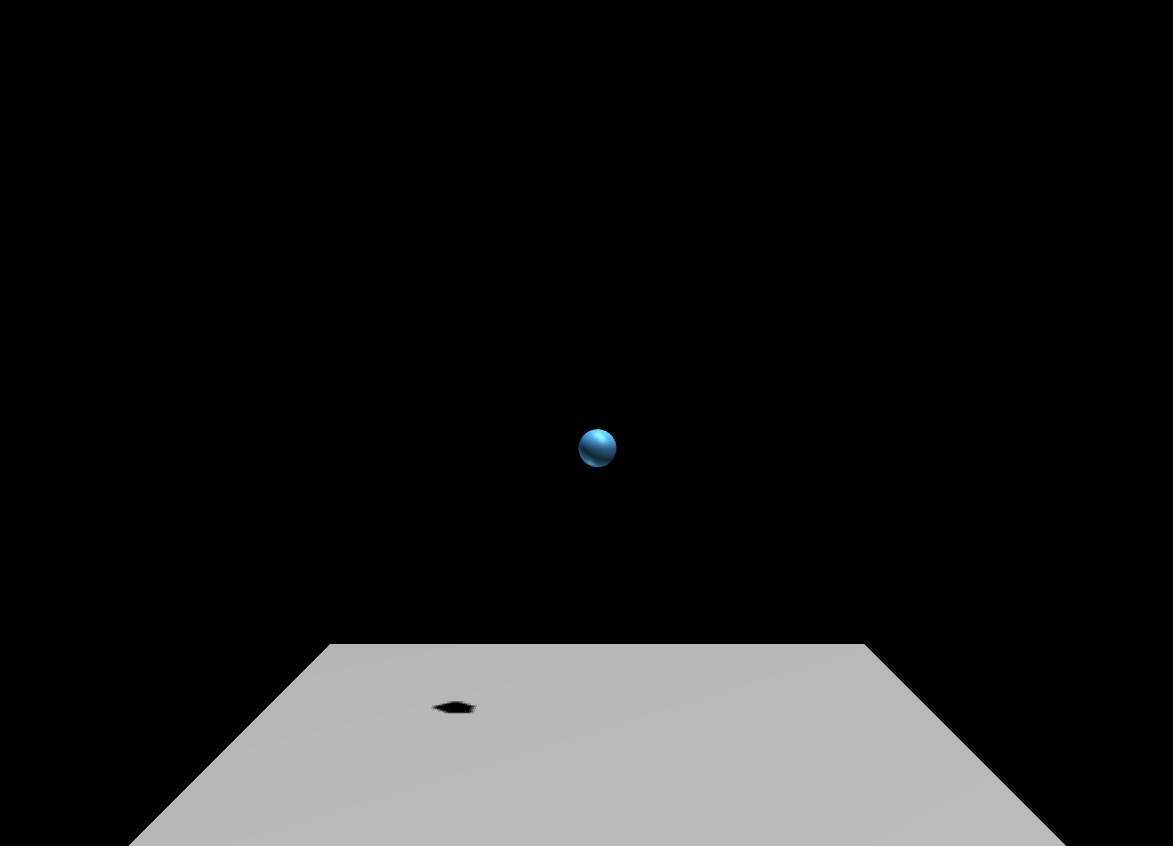
\includegraphics[width=0.5\linewidth]{images/simulation/simulation_js.png}
   \caption{three.js環境下でのシミュレーションの様子}
   \label{fig:simulation_js}
\end{figure}

また次に図\ref{fig:result_graph_js}として，このシミュレーションの時系列データのグラフを示す．高さが$0m$に達する前にバウンドしており，その高さは回数を重ねるごとに低くなっていることが確認できる．

\begin{figure}[htbp]
   \centering
   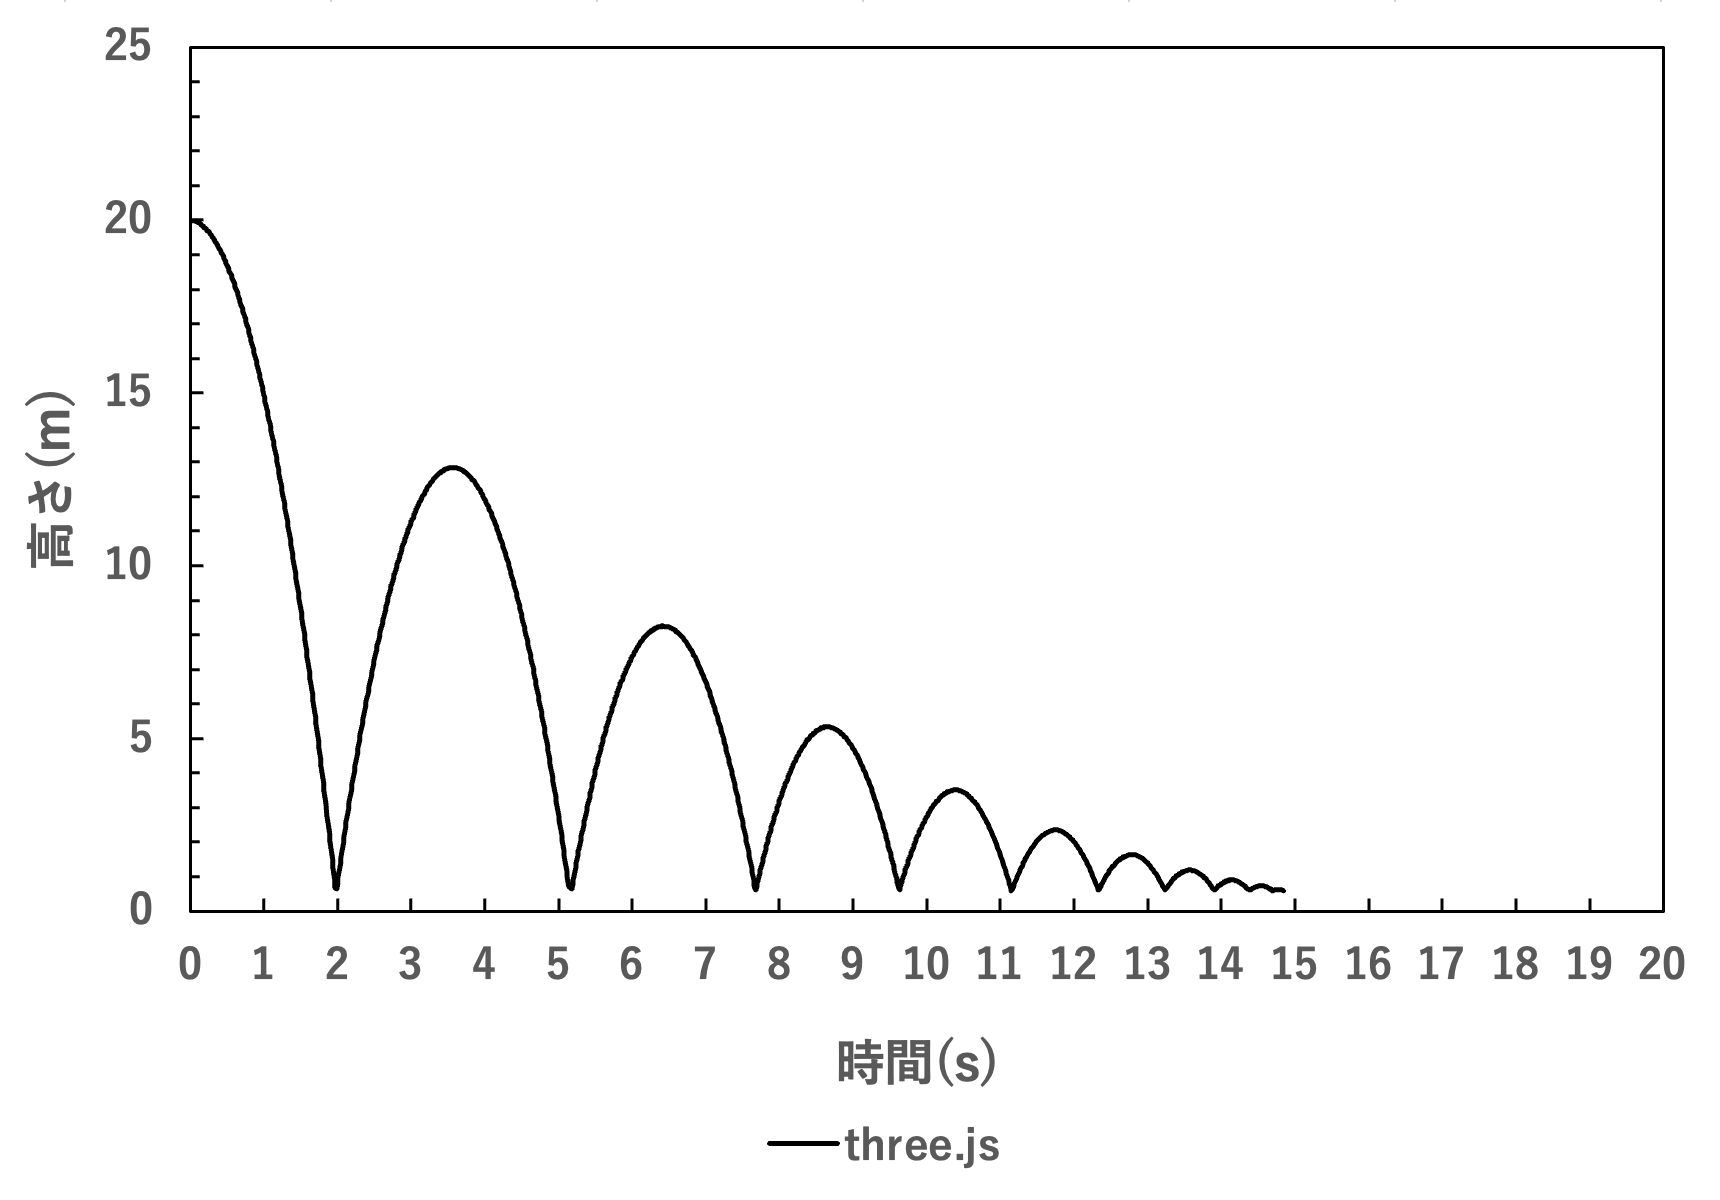
\includegraphics[width=0.75\linewidth]{images/simulation/result_graph_js.png}
   \caption{three.js環境下での自由落下シミュレーションの結果}
   \label{fig:result_graph_js}
\end{figure}

\begin{figure}[htbp]
   \centering
   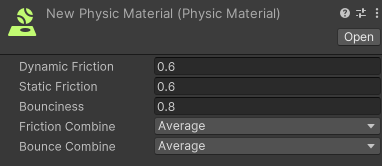
\includegraphics[width=0.75\linewidth]{images/simulation/unity_material.png}
   \caption{反発係数を0.8としたマテリアルの作成}
   \label{fig:unity_material}
\end{figure}

\subsection{Unityでの物理シミュレーションの記述方法と実装結果}
\ifdraft
この節では球の落下と衝突のシミュレーションについて、Unityでの実装の方法について、スクリーンショット図表、コードの一部を交えて説明する。また結果のCGのスクリーンショット、さらに、球の落下を示すシミュレーションの結果を時系列のグラフで示し、その特徴を論述する。

ここでは2.2節と同様のフォーマットでグラフなどを準備することが好ましい。同様のフォーマットとは時間範囲や単位を揃え、2つのグラフを比較可能にするという意味である。
\fi
% 以下に本文を書く
2.2節では物理エンジンであるUnityを用いた球体の落下と衝突のシミュレーションについて，その実装方法を解説する．使用したUnityのバージョンは2022.3.62f3である．この環境においてJavaScriptでのシミュレーションと同様に，床面から20m離れた空中に直径1mの球体を配置した．球体に物理的な重力挙動を与えるために，RigidBodyコンポーネントを追加した．ここで与えられる重力加速度は，Unityの初期設定通りである9.81$m/s^2$である．さらに球体のバウンドを再現するために，図\ref{fig:unity_material}に示すような反発係数を0.8としたマテリアルを作成し，これを球体と床面の双方のオブジェクトに適応した．これによって球体は床面に衝突した際にバウンドするようになった．これに加えシミュレーション結果の時系列データを数値的に得るために，時間毎の球体の高さを記録しcsvファイルとして出力するスクリプトを球体オブジェクトに付与した．このような環境下で実施したシミュレーションの様子を図\ref{fig:simulation_unity}として示す．灰色の球体が地面に向かって自由落下する様子が確認できる．

\begin{figure}[htbp]
   \centering
   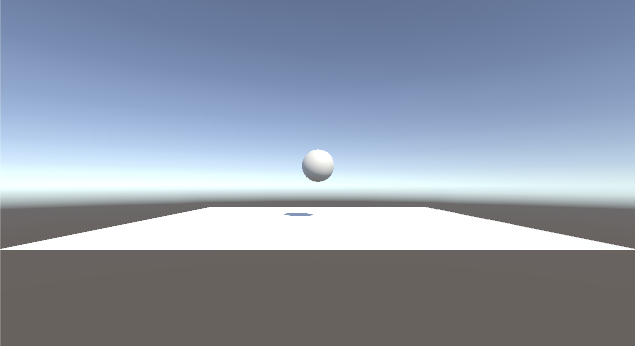
\includegraphics[width=0.75\linewidth]{images/simulation/simulation_unity.png}
   \caption{Unityを用いた自由落下シミュレーションの様子}
   \label{fig:simulation_unity}
\end{figure}

また次に図\ref{fig:result_graph_unity}に示すのは,このシミュレーションの時系列データのグラフである．高さ$0m$に近い地点でバウンドしており，JavaScriptを用いた時と同様に，バウンドするたびに達する高さの最大値は小さくなっている．

\begin{figure}[htbp]
   \centering
   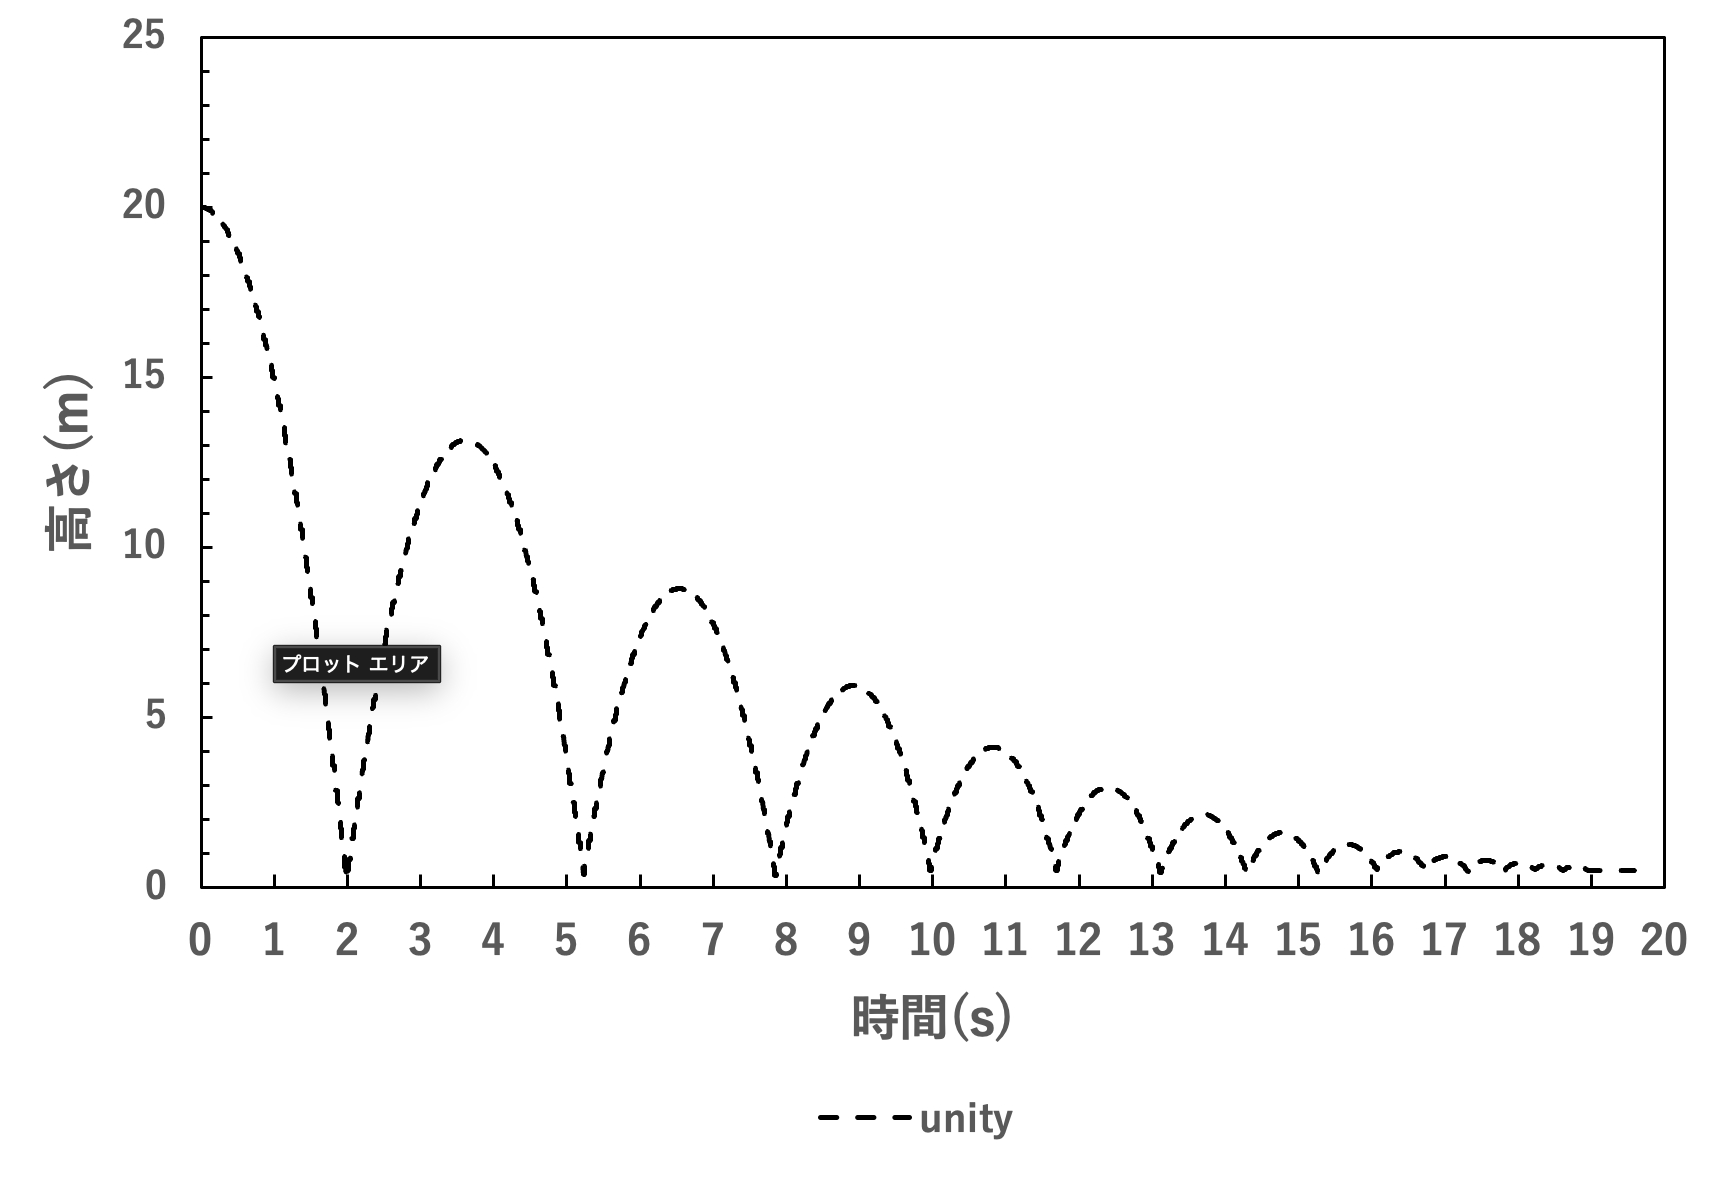
\includegraphics[width=0.75\linewidth]{images/simulation/result_graph_unity.png}
   \caption{Unityを用いた自由落下シミュレーションの結果}
   \label{fig:result_graph_unity}
\end{figure}


\subsection{シミュレーション結果と解析解との比較検討}
\ifdraft
この節では、\textbf{最初の衝突までの落下挙動}について、(1) JavaScriptのシミュレーション結果、(2) Unityでのシミュレーション結果を、(3) 物理学で学習した物体の落下運動方程式から解析的に得た理論値とそれぞれ比較して、シミュレーションの精度について考察する。

ここで言及する精度とは、単に表示の桁数の大小ではなく、まず3つの計算結果を一つのグラフにまとめて統合し、そのうえで(3)の解析解と、(1),(2) のシミュレーション結果との差異を誤差として検証し、客観的に結果を評価すること。評価ポイントは以下である。
\begin{itemize}
    \item 正解としての解析的に得た論理値の導出方法について式を明記して導出方法と導出結果を記載すること
    \item それらが乖離する場合には、なぜそのような結果が出たかを考えて、自分の解釈を論理的に述べること。単に``似ている''、``近い''、``良い''ではなく，数値として精度を評価し，シミュレーションの目的を踏まえてその誤差について述べる
    \item 特に各シミュレーションでの結果は、物理現象としての``初期値''がどのように設定されているかが、シミュレーション結果を比較する上で極めて重要なポイントである
    \item 論述文において、配布したテキストや講義ウェブページからのコピーは剽窃と見なす
\end{itemize}
\fi
% 以下に本文を書く
2.3節において，まず初めに理論値の導出方法を示す．時間tにおける球体の高さをyとおき，これを
\begin{equation} \label{eq:set_y}
    y=y(t)
\end{equation}
 とする．$y(t)$は時刻tにおける初期地点からの落下距離であるため，両辺を時間で微分することにより，時刻tにおける速度は，
\begin{equation} \label{eq:set_v}
    v(t)=\frac{dy(t)}{dt}
\end{equation}
さらに時間で微分することで，加速度は，
\begin{equation} \label{eq:set_a}
    a(t)=\frac{dv(t)}{dt}=\frac{d^2y(t)}{dt^2}
\end{equation}
と表される．球体の質量を$m$とおくと，球体にかかる力は重力加速度を$g$として$mg$で表されるため，これらを運動方程式に代入すると，
\begin{equation} \label{eq:EOM1}
    ma(t)=mg
\end{equation}

\begin{equation} \label{eq:EOM2}
    \frac{d^2y(t)}{dt^2}=g
\end{equation}

この(\ref{eq:EOM2})の微分方程式を解くことによって(\ref{eq:freefall_gen})に示す自由落下の式を得た．

\begin{equation} \label{eq:freefall_gen}
    y=\frac{1}{2}gt^2+v_0t+y_0
\end{equation}

今回のシミュレーションは高さ$20m$からの自由落下であるため，この運動を示す指揮は次の(\ref{eq:freefall})に示す通りである．

\begin{equation} \label{eq:freefall}
    y=20-\frac{1}{2}gt^2
\end{equation}

この式(\ref{eq:freefall}) において1回目の衝突時，即ち$y=0$とした時の時間$t$の値は，
\begin{equation} \label{eq:freefall_0}
    0=20-\frac{1}{2}gt^2
\end{equation}
より
\begin{equation} \label{eq:freefall_answer}
    t\simeq2.02
\end{equation}
であった．(重力加速度は9.81として算出した．)

図\ref{fig:result_graph_all}に示すのは，上記のthree.jsを用いたシミュレーションとUnityを用いたシミュレーションの双方の結果の，0秒から1回目の衝突後までの範囲をプロットしたグラフである．また次の図\ref{fig:result_graph_collision}に示すのは，図\ref{fig:result_graph_all}における1回目の衝突の前後を拡大したグラフである．ここでUnityの結果が階段状になっているのは，ログを出力するスクリプトにおけるUpdate関数の更新頻度はデバイスのフレームレートに依存し，その頻度が物理シミュレーションの計算間隔よりも短いことに起因している\cite{unityUpdate}．three.jsのアニメーションの更新間隔は0.01秒，Unityのシミュレーションの計算間隔は初期設定の0.02秒であるため，グラフのメモリは0.01秒刻みで描いている．

\begin{figure}[htbp]
    \centering
    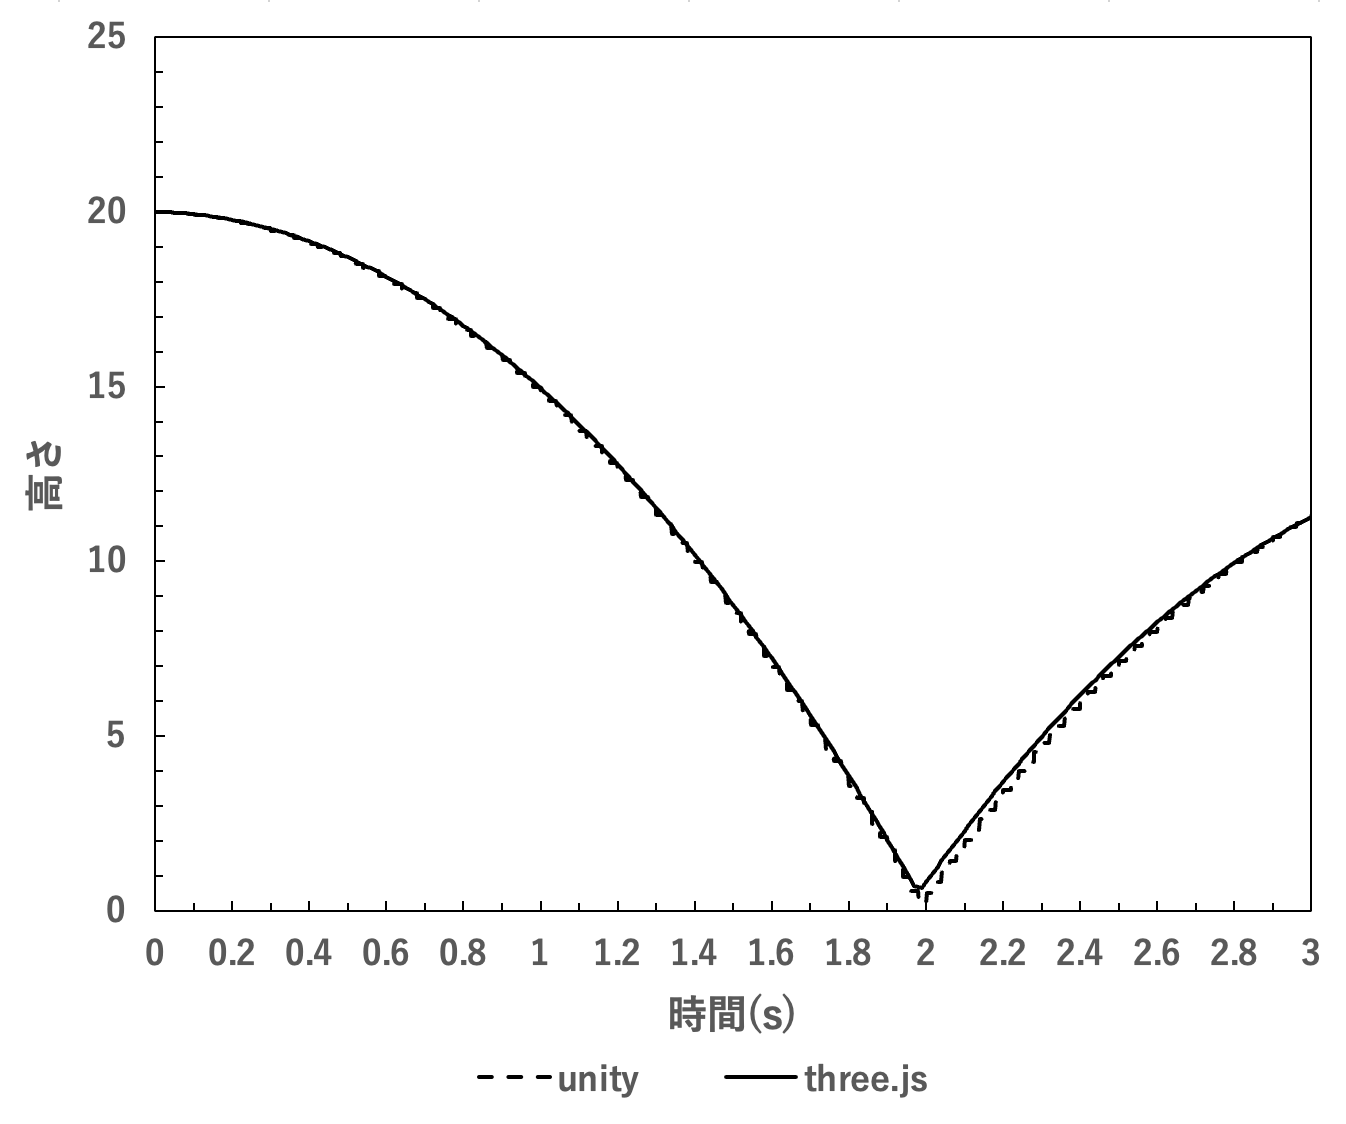
\includegraphics[width=0.75\linewidth]{images/simulation/result_graph_all.png}
    \caption{自由落下シミュレーション結果の集計}
    \label{fig:result_graph_all}
\end{figure}

\begin{figure}[htbp]
    \centering
    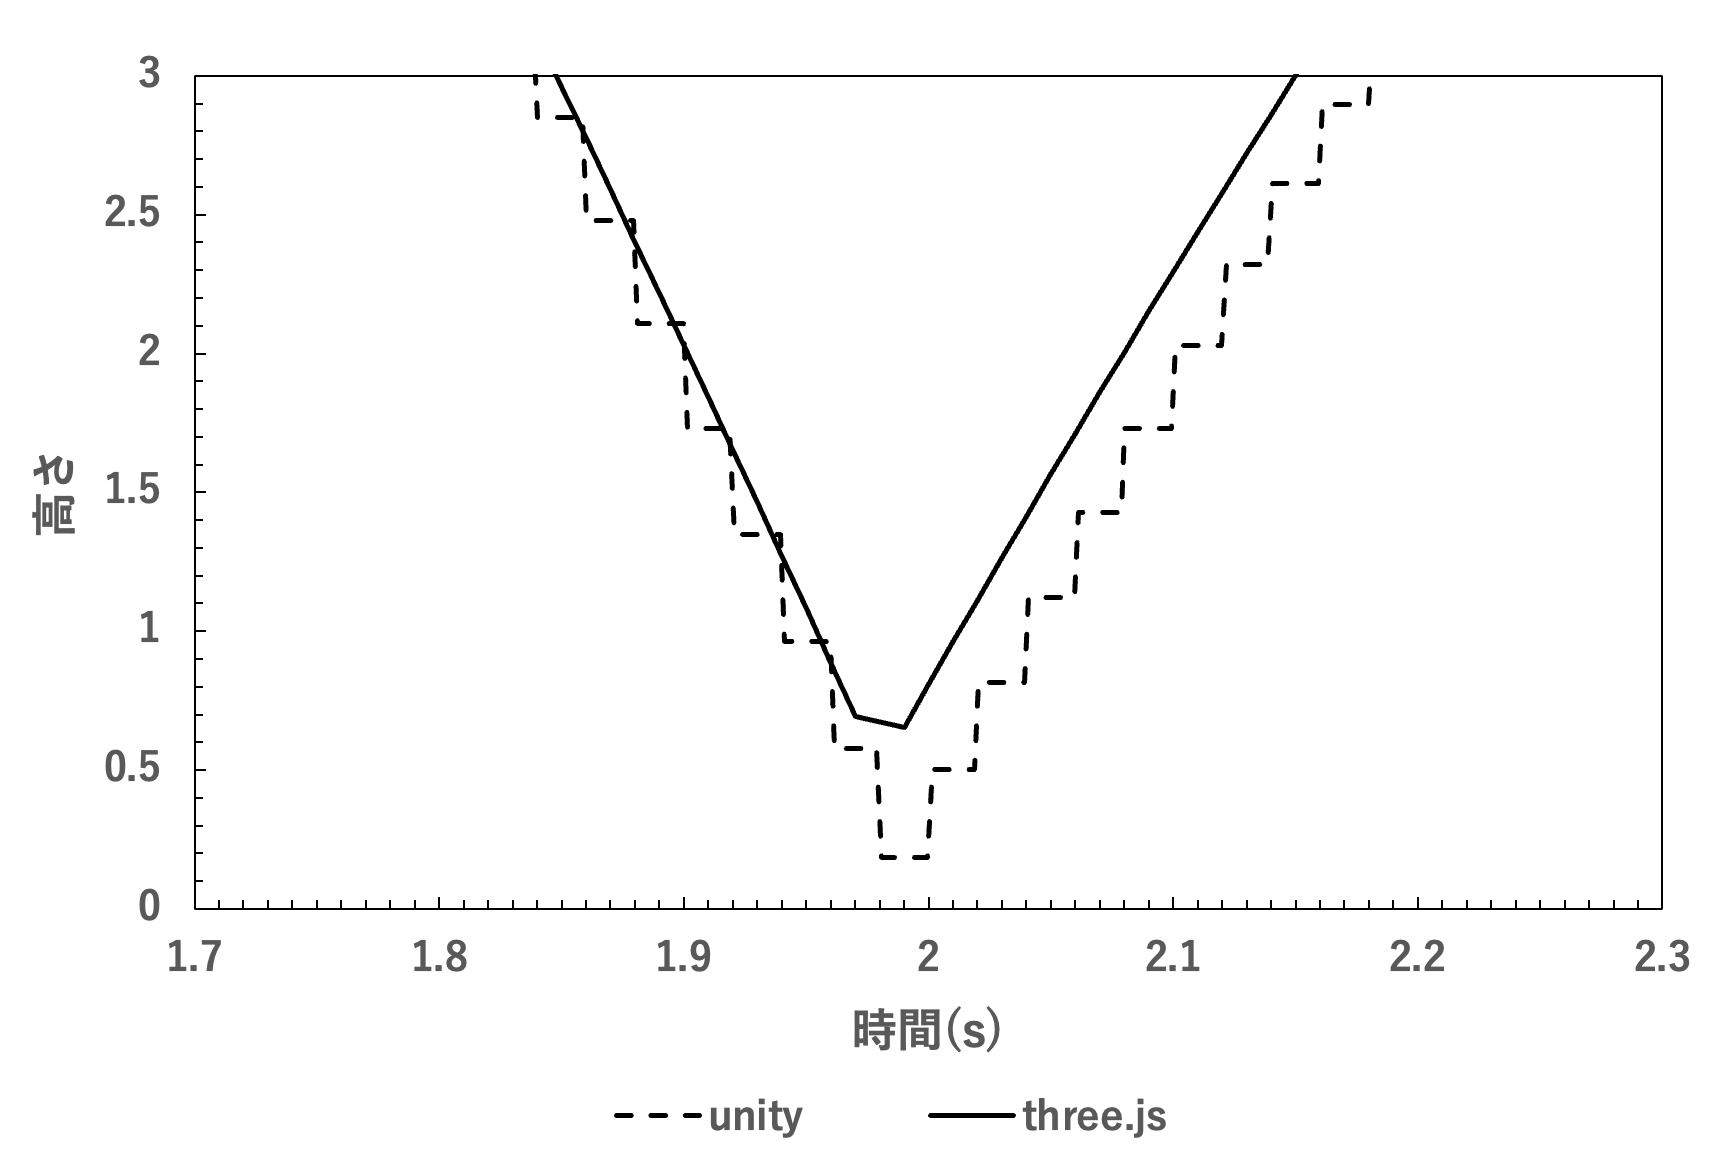
\includegraphics[width=0.8\linewidth]
    {images/simulation/result_graph_collision.png}
    \caption{自由落下1回目の衝突前後}
    \label{fig:result_graph_collision}
\end{figure}

three.jsを用いたシミュレーションでは，球体の高さを次に示す式(\ref{eq:velociy}),(\ref{eq:hight})で計算している．

\begin{equation} \label{eq:velociy}
    v_{n+1} = v_n + gΔt
\end{equation}

\begin{equation} \label{eq:hight}
    y_{n+1} = y_n + v_{n+1}Δt
\end{equation}

球体の床面との衝突判定条件は$y_n < 0.5$と設定したため，式(\ref{eq:velociy}),(\ref{eq:hight})によれば，$n=198$,即ち$1.98(s)$で球体の中心座標は$y=0.498(m)$の時に衝突したと判定されるはずである．しかし先に示した出力のコードによると，この時の中心座標はコンソールに出力されるための条件を満たしていない．したがって図\ref{fig:result_data_js}に示す衝突前後のデータで示されるように，時間$1.98(s)$のデータが存在せずその計算結果を無視し，$1.99(s)$のデータが出力されている．

\begin{figure}[htbp]
    \centering
    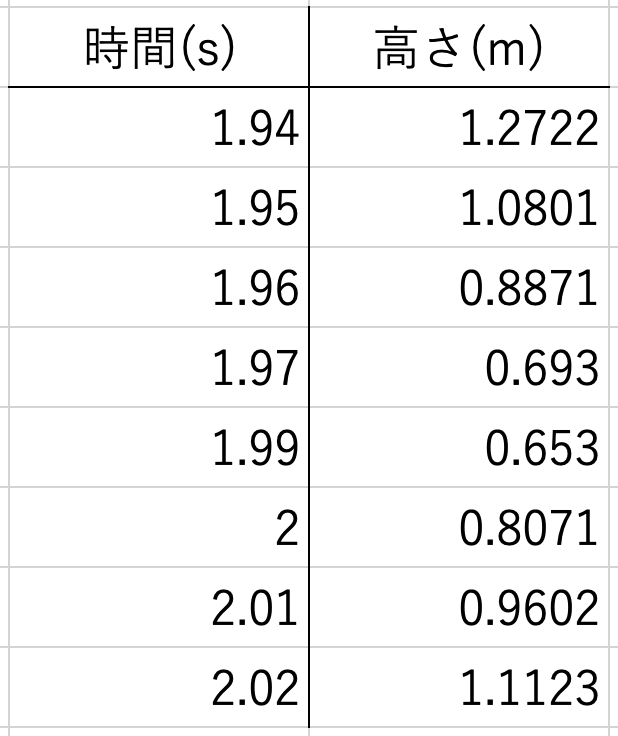
\includegraphics[width = 0.3 \linewidth]
    {images/simulation/result_data_js.png}
    \caption{thrree.jsシミュレーションの衝突前後のデータ}
    \label{fig:result_data_js}
\end{figure}

次にUnityを用いたシミュレーションでは，計算間隔は0.02秒で指定しているが，これはthree.jsでのシミュレーションと比べるとその更新頻度は半分である．ここでthree.jsのシミュレーションで用いた計算式(\ref{eq:velociy}),(\ref{eq:hight})を用いて計算すると，$n=99$, $1.98(s)$の時に$y=0.60(m)$を得て，$n=100$, $2,00(s)$の時に$y=0.20(m)$を得る．この結果は図\ref{fig:result_graph_collision}のグラフから読み取れるように，高さ$y=0.20(m)$に到達した時に衝突の判定がなされていることを意味している．

この２つのシミュレーション間の結果に差があるのは，計算間隔が異なることに起因していると考え，これについて検証していく．three.jsでは計算間隔が$0.01(s)$であったため，Unityの計算間隔も同じ$0.01(s)$にしてシミュレーションをした結果を図\ref{fig:result_simlation}に示す．この図に示されるように，計算結果がほとんど一致していることが分かる．なおunityの結果のサンプリング数が多いのは，計算間隔よりも画面の更新間隔の方が短いためである．また解析解で得られた，式(\ref{eq:freefall_answer})との差については，これらのシミュレーションの記録が，プログラム実行時点と同時に始まっておらず時間軸にずれが生じているためであると考えた．

\begin{figure}
    \centering
    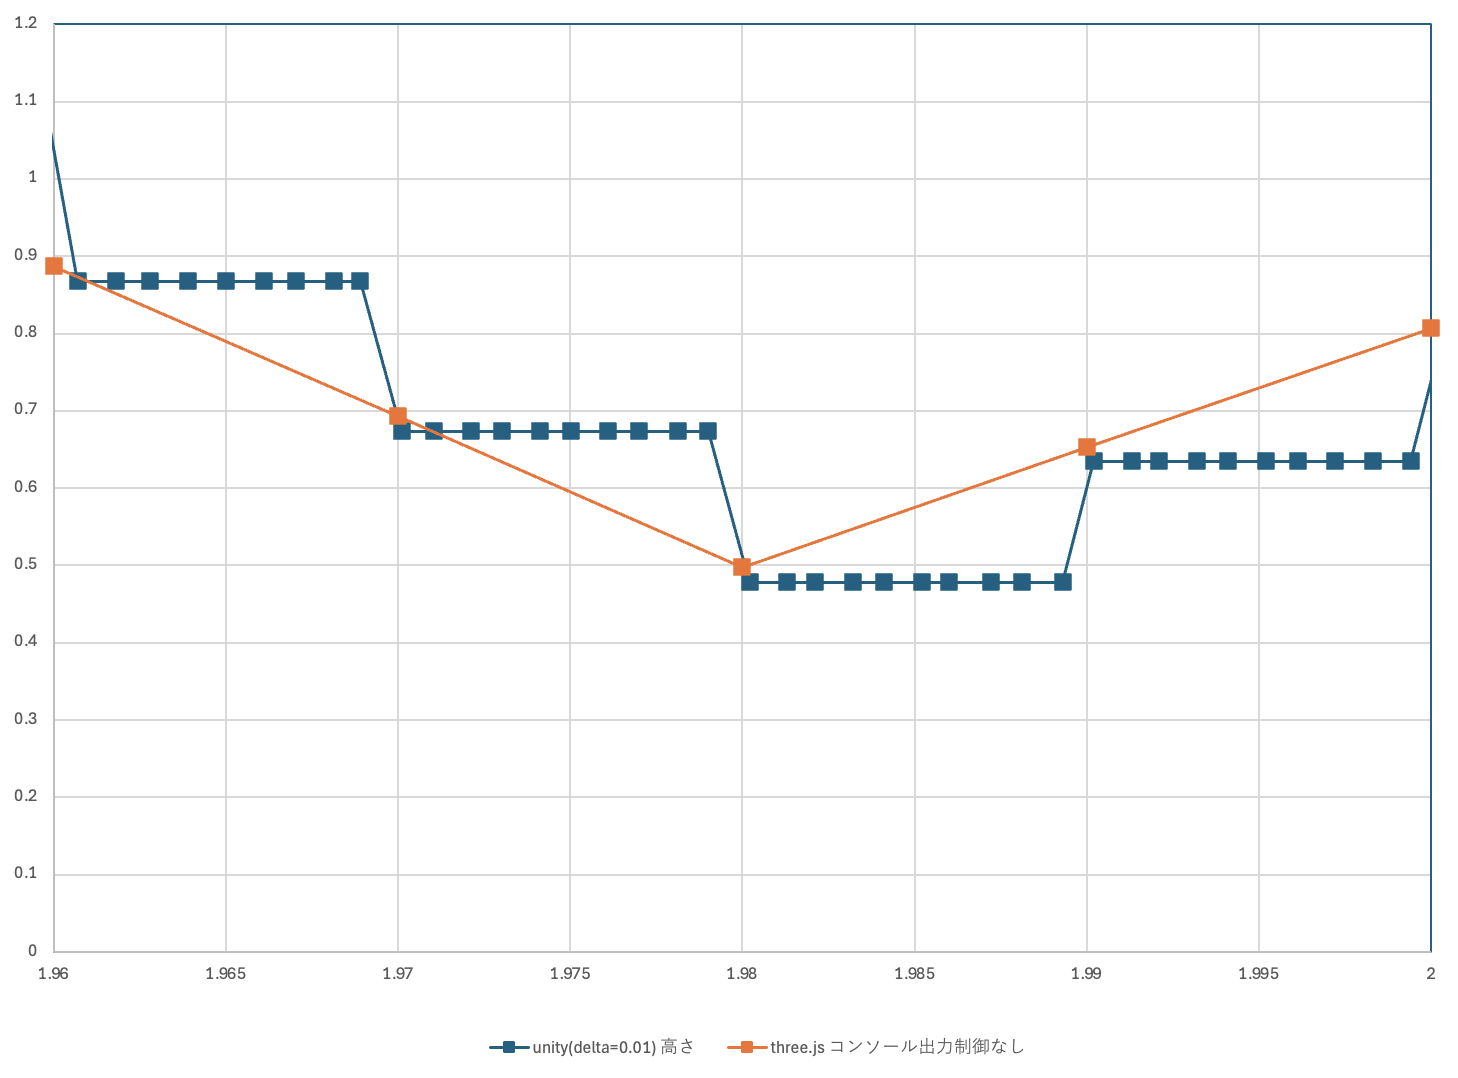
\includegraphics[width=0.75\linewidth]{images/simulation/result_simulation.png}
    \caption{検証結果}
    \label{fig:result_simlation}
\end{figure}

\section{制作した課題作品の構想}
\ifdraft
各グループで構想した課題作品の概要について、班内でまとめたアイデアスケッチを添えて述べる。
なお、この実験のレポートの最後では、この構想に対して実現できた部分、実現できなかった部分を議論する。その際に実現したものとできなかったものを明確に区別するために、アイデアスケッチを用いて具体的に実現を目指す内容を論述すること。

具体的には、作品タイトル、作品のシナリオ、開発する仮想空間や、その中でのユーザの体験の説明など、制作を目指した作品についての詳細について説明する。ここで、\textbf{必ず講義中に書いたアイデアスケッチを十分な解像度で添付する}こと。単にスマートフォンなどで写真を撮影したものではなく、適切な画像処理を施して読めるようにせよ。

同じ班の中で、スケッチ図面を共有することは認める。ただし、図面の著作者を図面毎に明記し、説明の文書は各自で自分の文書を作成すること。複数人の論述文が一致する場合は、剽窃と見なす。テキストや講義Webページからのコピーも剽窃と見なす。
\fi
% 以下に本文を書く
制作する作品のタイトルは「SPACE SORT」である．この作品は未来の人類が宇宙空間での生活を営んでいると仮定し，その際に生じる荷物の運搬作業を遠隔操作するロボットによって行うことを想定している．ユーザはHMDを装着することでその空間を擬似体験することができ，頭部の動きに合わせて視界が変化する．同様に手の動きをコントローラのセンシングによってVR空間にリンクさせ，ロボットの手を動かす．自身がロボットを１人称視点から操作することを体験するものである．宇宙空間である事を活用した３次元的な動きが可能であることや，重力の影響がないことで物体が地球上とは異なる挙動となることを体験できるのが，この作品の特徴である．またゲーム性を持って体験できるように，荷物を正しく運ぶことによるポイントの加算や，ロボットのバッテリー管理を必要とするシステムにするなどしている．イメージスケッチを図\ref{fig:pj_image1},\ref{fig:pj_image2}に示す．

この作品を制作するにあたっての私の役割は，モデラとして3Dモデルを制作することである．主にプレイヤーが操作するロボットを作成し，単にモデルを作成するだけでなくボーンを入れることで，Unityにおけるモデルの動作を容易にさせることを目標にする．またUnityの中で動作させることから，できる限り計算コストを小さくするために，最小限のポリゴン数で構成されるように配慮する．

\begin{figure}[htbp]
    \centering
    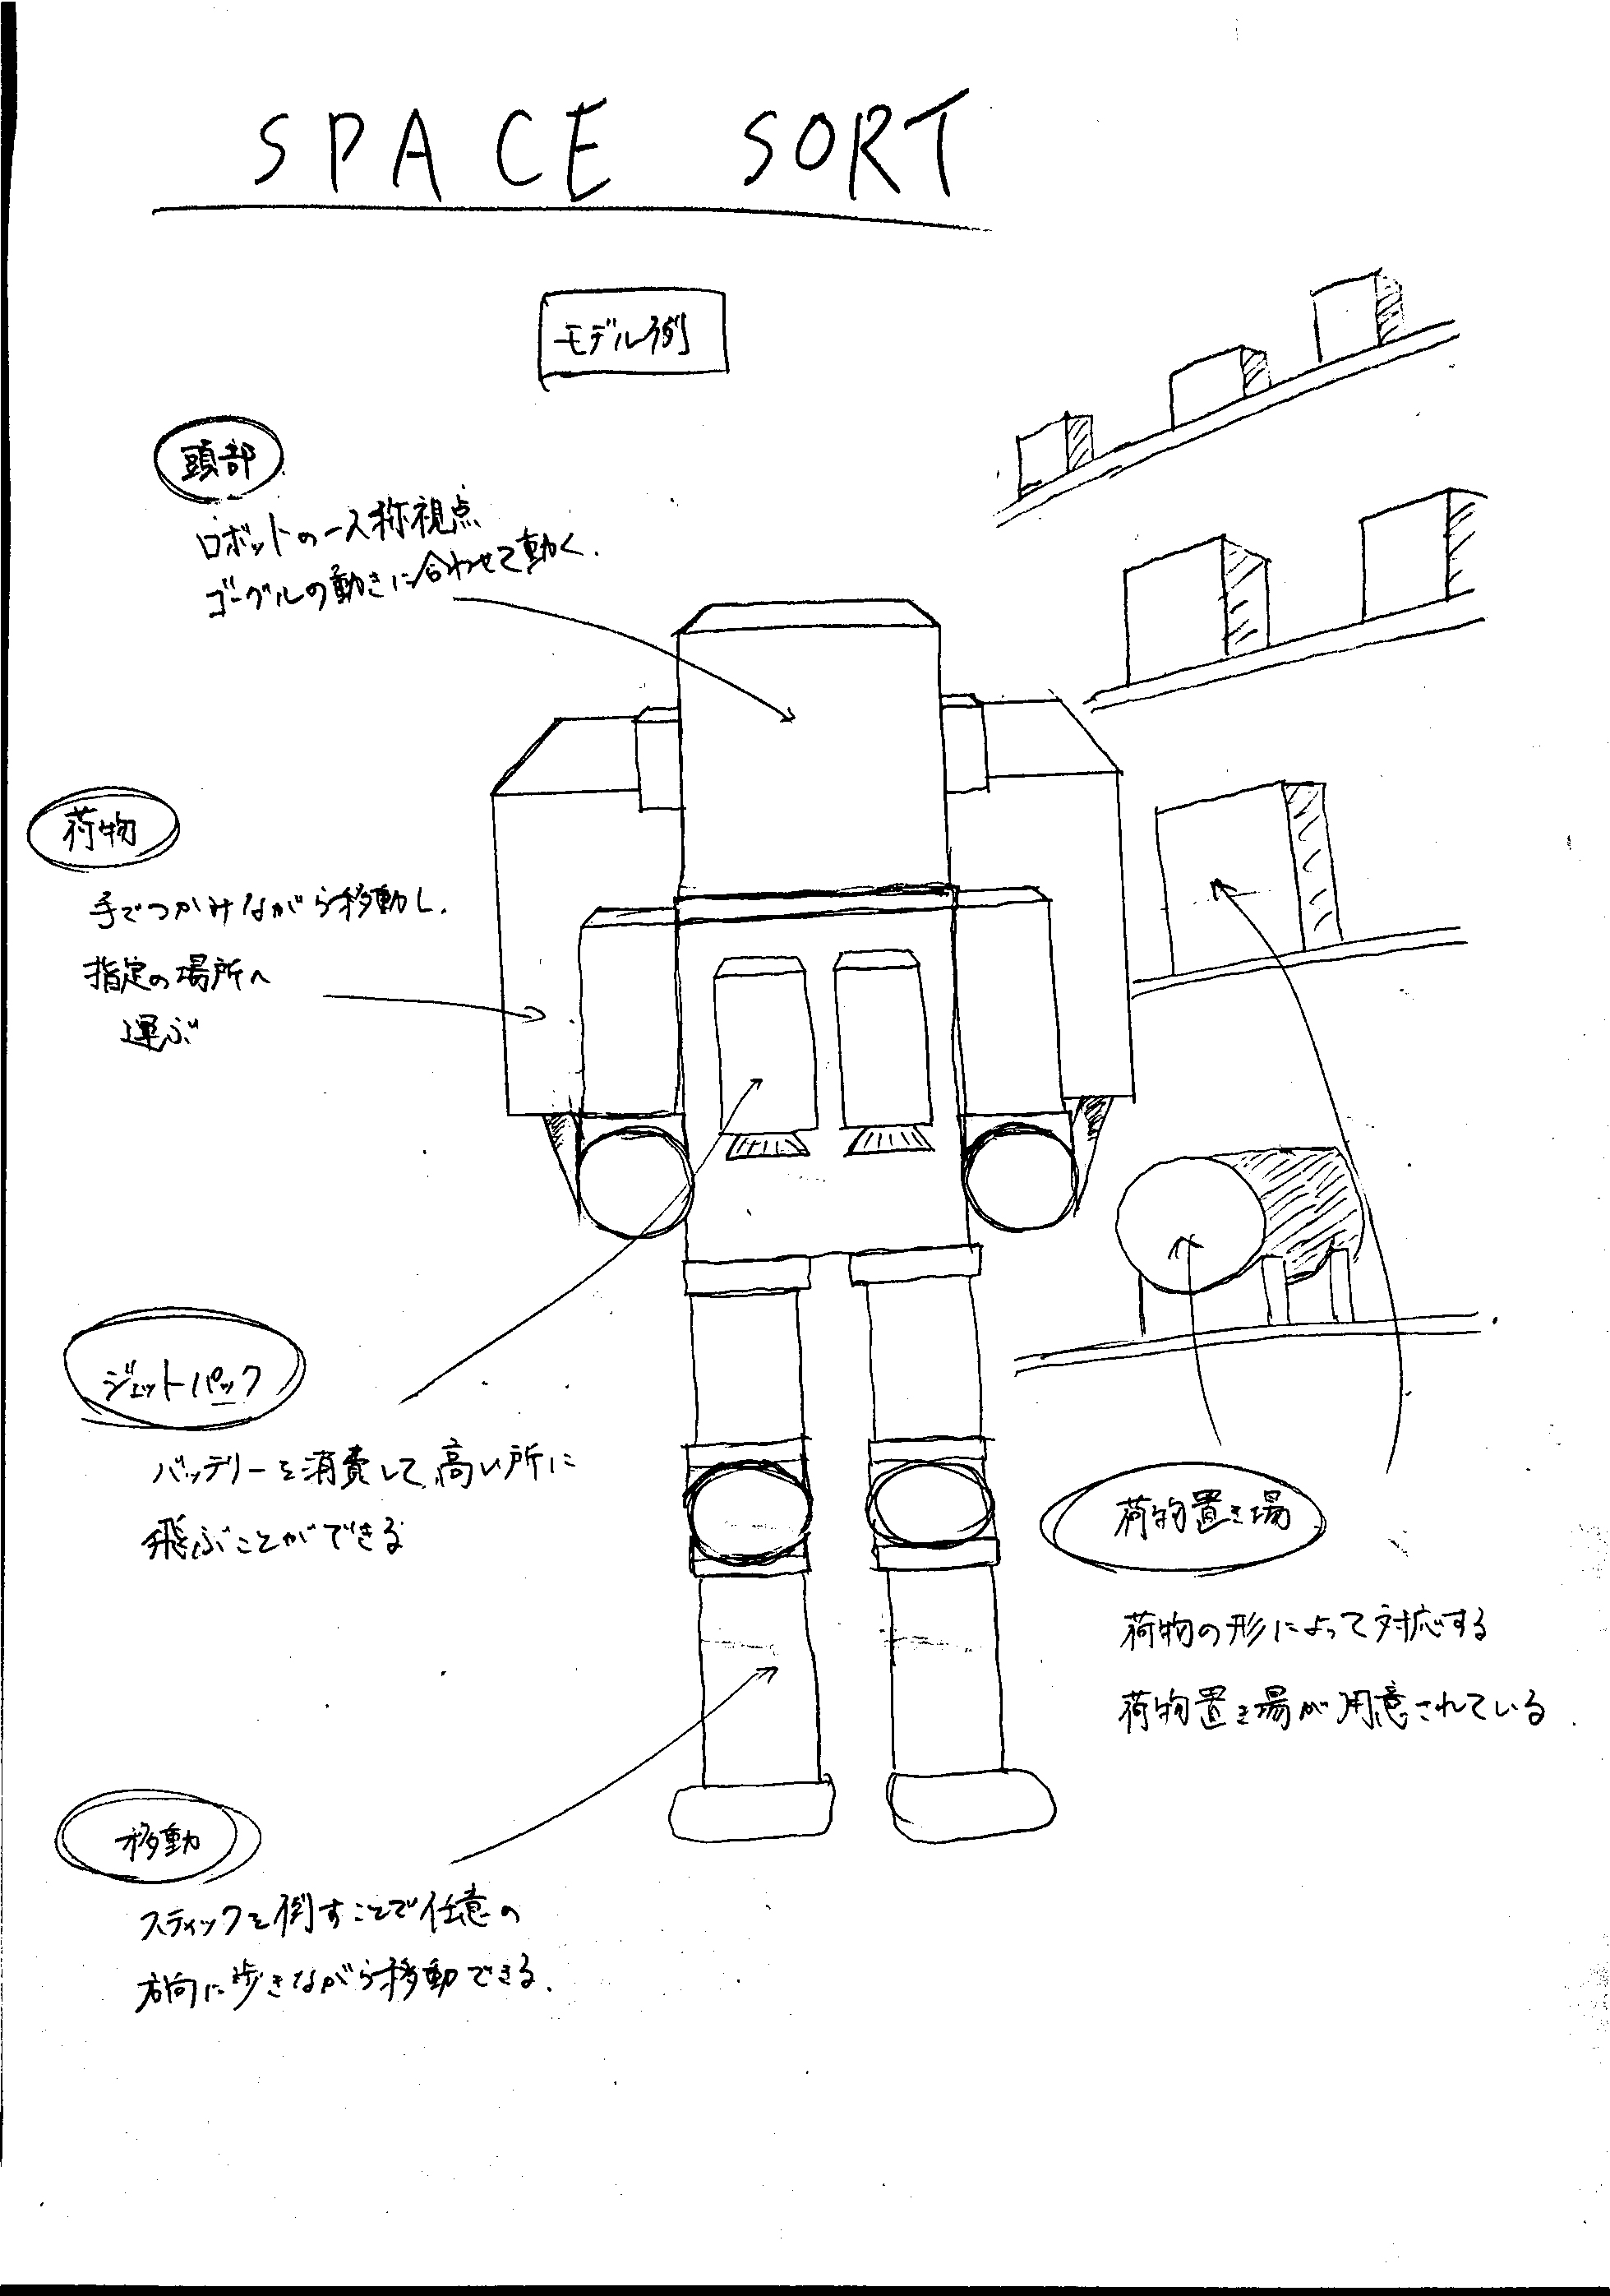
\includegraphics[width=0.85\linewidth]{images/pj_image1.jpg}
    \caption{アイデアスケッチ１：}
    \label{fig:pj_image1}
\end{figure}

\begin{figure}[htbp]
    \centering
    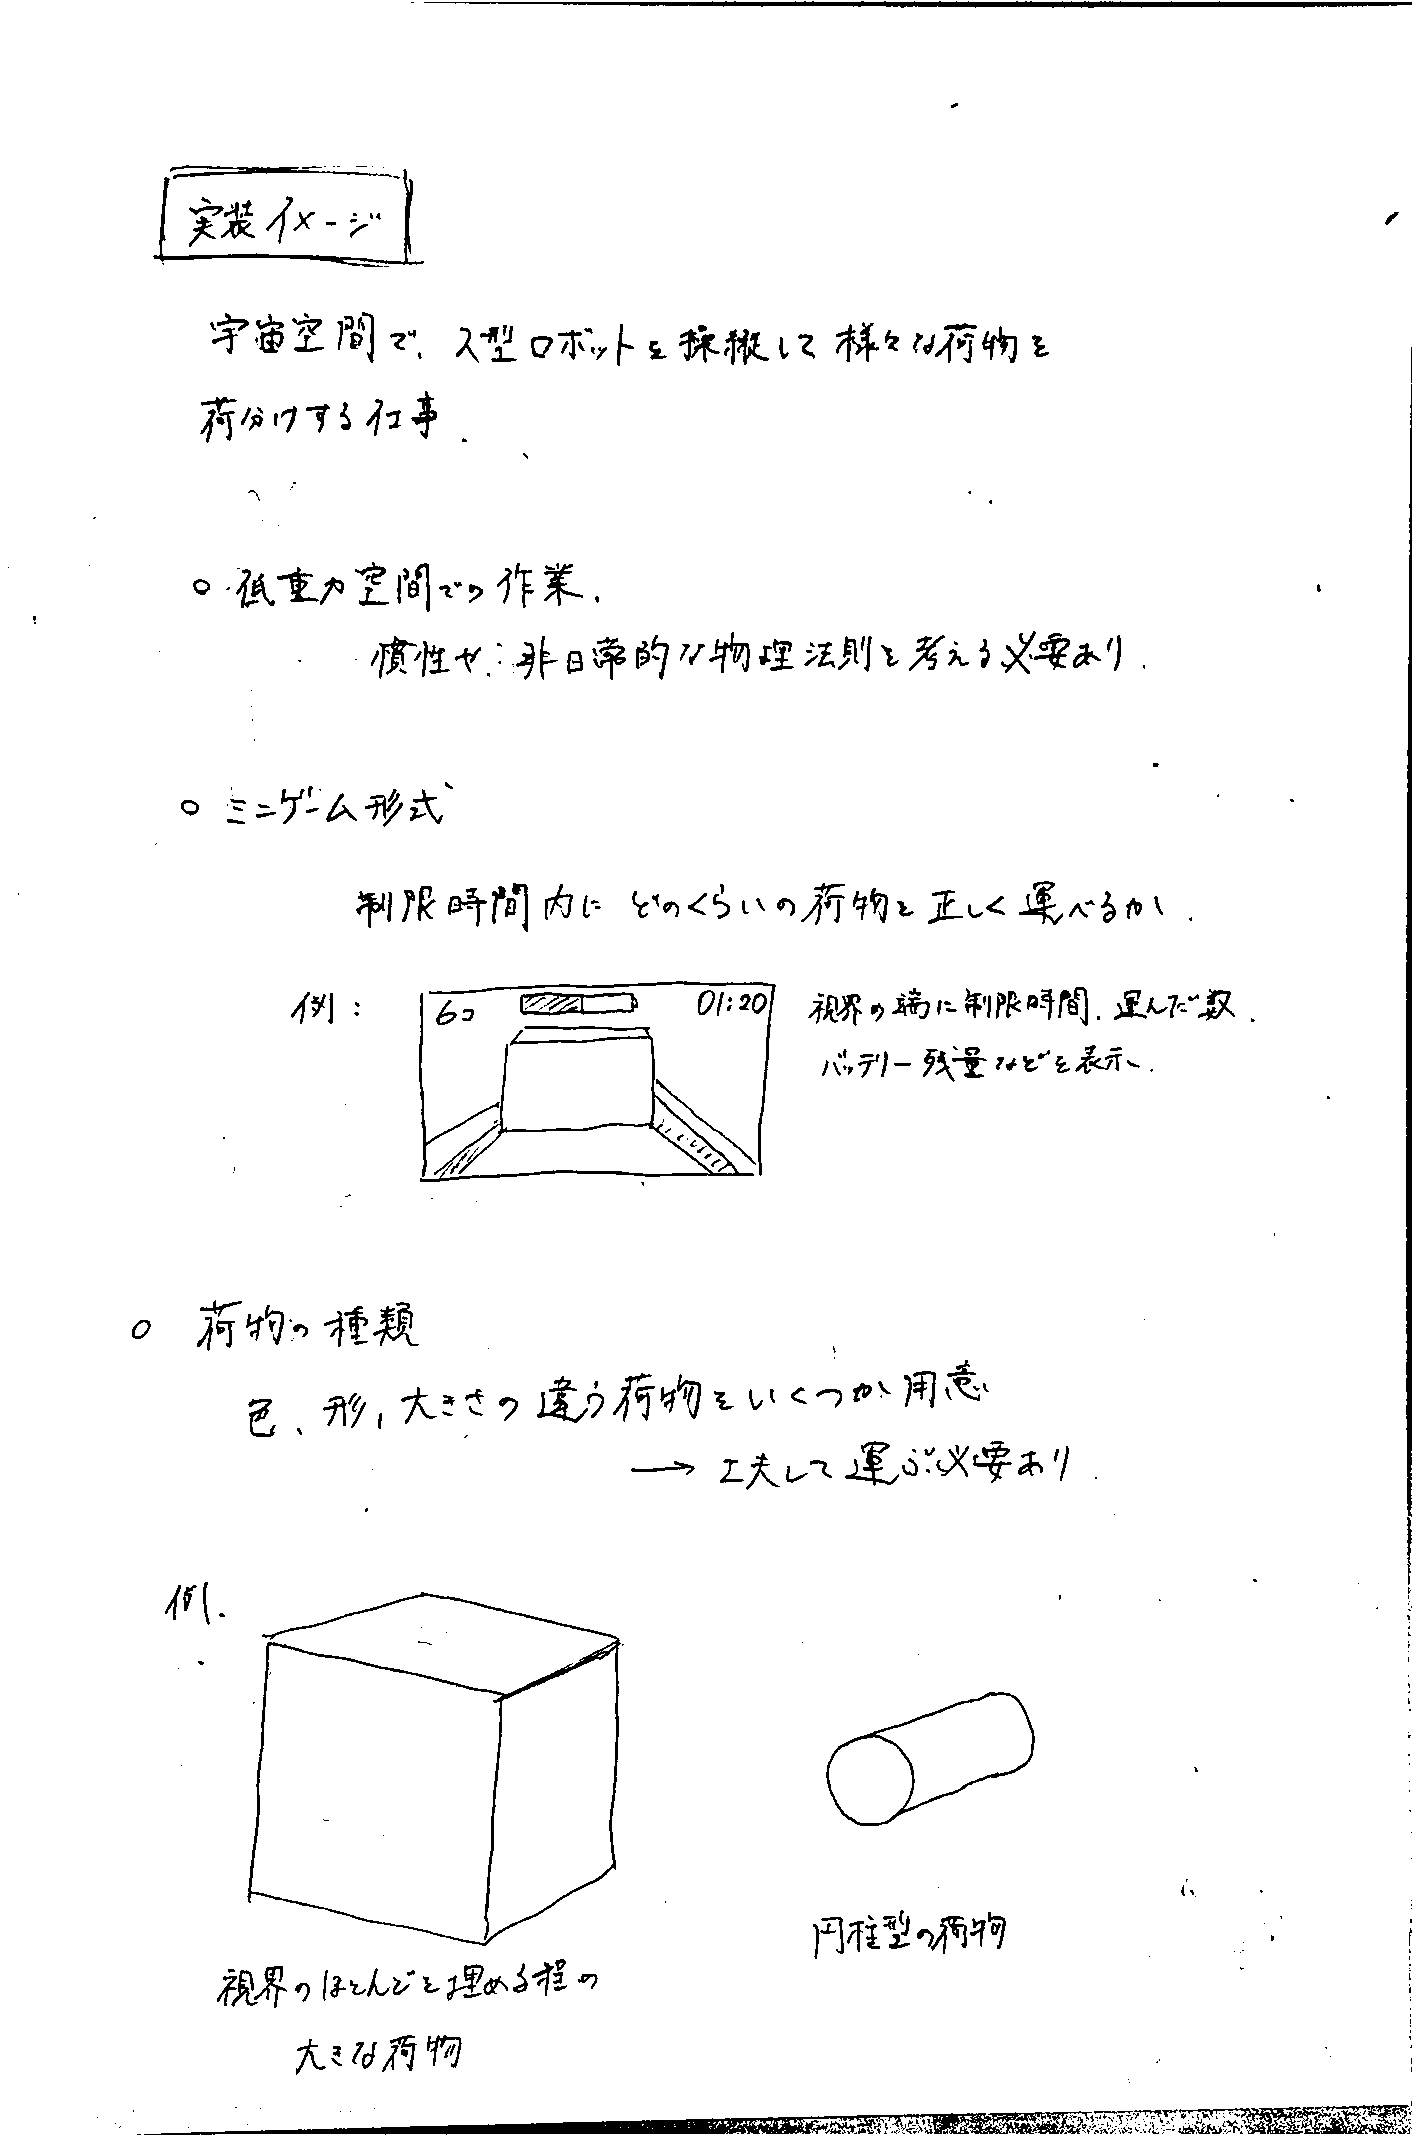
\includegraphics[width=0.85\linewidth]{images/pj_image2.jpg}
    \caption{アイデアスケッチ２}
    \label{fig:pj_image2}
\end{figure}




\section{作品における課題と解決方法}
\ifdraft
作品における課題について計画、達成するべき課題などをまとめ、その課題を解決するためにどのような技術や機器を用いたのかを説明する。
\fi
% 以下に本文を書く
この作品を制作するにあたって，最低限実装するべき機能は以下の5点である．
\begin{enumerate}
    \item 歩行などのロボットのアニメーション \label{enu:animation}
    \item ユーザの装着するHMDやコントローラの動きとロボットの動きのリンク \label{enu:rink}
    \item ロボットの前後移動や上下移動を，低重力であることを念頭に置いて実現する \label{enu:move}
    \item 荷物を掴む機能 \label{enu:grab}
    \item 荷物を所定の場所に置いたときのゴール判定機能 \label{enu:goal}
\end{enumerate}
さらにここから，よりゲーム性を持たせるために，ジェットパックを使って飛行モーションに対して制限時間を設けることや，タイムアタック形式にしてランキングを表示する機能を実装する．

課題\ref{enu:animation}と\ref{enu:rink}に挙げたロボットのアニメーションやユーザの動きとのリンクについては，6章の担当作業内容で詳しく説明するが，blenderを用いて作成したモデルにUnityの標準形式のボーン構造を取り入れることで解決した．これを用いることによって，Unity側で複雑なアニメーション操作をすることなく，モデルに任意の動きを持たせることができる．課題\ref{enu:move}については，重力加速度の値を小さくすること，また歩行速度を遅めに設定することによって，移動に普段よりもふわふわとした印象を持たせるようにした．課題\ref{enu:grab}をクリアするためには，ユーザの手の動きから仮想空間上のロボットの手の位置を決定し，その位置と荷物の距離が一定値以下かつコントローラからの入力があったときに荷物を手の位置に吸着するように動かすことができるようにスクリプトで設定した．課題\ref{enu:goal}についても同様に，スクリプトによりゴール範囲内に荷物が置かれたときに設置判定を出すようにした．

またゲーム性を持たせるために実装したジェットパックの制限時間についても，スクリプト上で飛行時間の管理を行った．ランキングの表示は使用したMetaQuest本体のファイルに上位3位までの記録を書き込むことでデータを引き継げるようにした．


\section{構築した課題作品の構造}
\ifdraft
まず、構築した作品の処理の流れを述べる。シーンの切替や、ユーザの行動をどのような機器で、どのように計測したのかについて述べる。また、その計測結果が仮想空間内の各オブジェクトにどのように影響を与え、変化するかについて、図表を交えて説明する。特に図表は\mbox{図\ref{fig:flow}}のフロー図のように図示することが望ましい。

また、仮想空間で構築したHierarchy構造についても図示し、それぞれのオブジェクトに組み込んだスクリプトについても機能を説明する。Hierarchy構造は\mbox{図\ref{fig:scenegraph}}のシーングラフ構造のように図示する。

同じ班の中で、図面を共有することは認めるが、説明の文書は各自で自分の文書を作成すること。論述文が一致する場合は、剽窃と見なす。

\begin{figure}[htb]
    \centering
    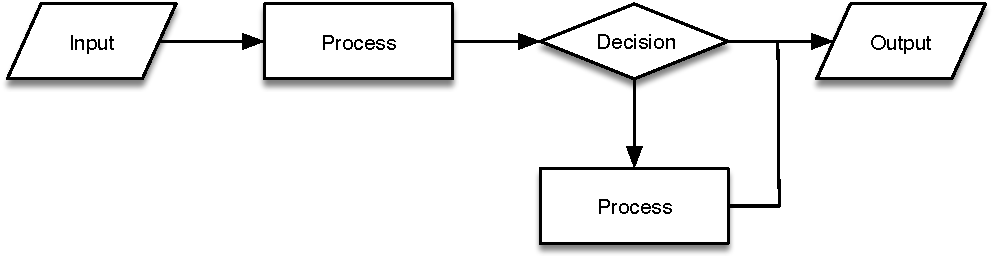
\includegraphics[width=0.7\linewidth]{images/flow.pdf}
    \caption{フロー図}
    \label{fig:flow}
\end{figure}

\begin{figure}[htb]
    \centering
    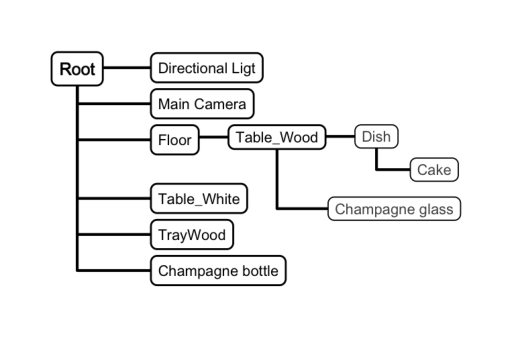
\includegraphics[width=0.7\linewidth]{images/scenegraph.pdf}
    \caption{シーン構造}
    \label{fig:scenegraph}
\end{figure}
\fi
% 以下に本文を書く
今回制作した課題作品のフローチャートを図\ref{fig:flow1},\ref{fig:flow2}に示す．\begin{figure}
    \centering
    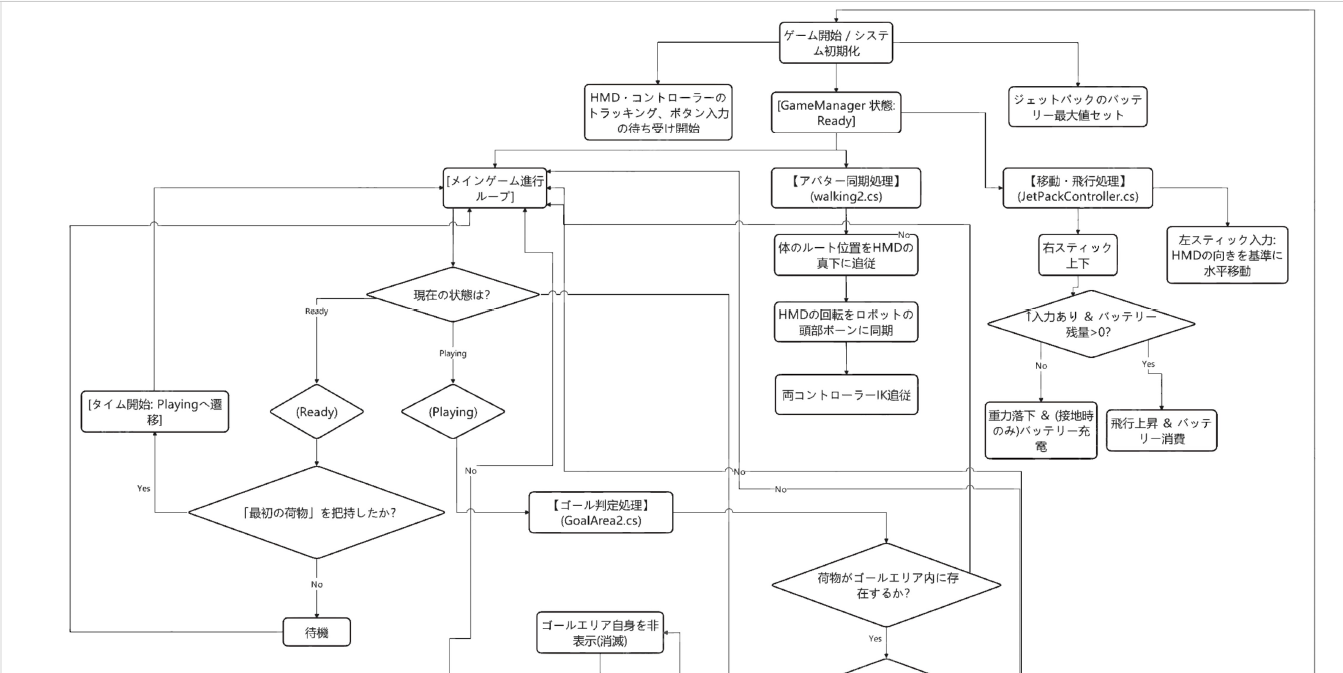
\includegraphics[width=1\linewidth]{images/flow1.png}
    \caption{フローチャート(１枚目)}
    \label{fig:flow1}
\end{figure}

\begin{figure}
    \centering
    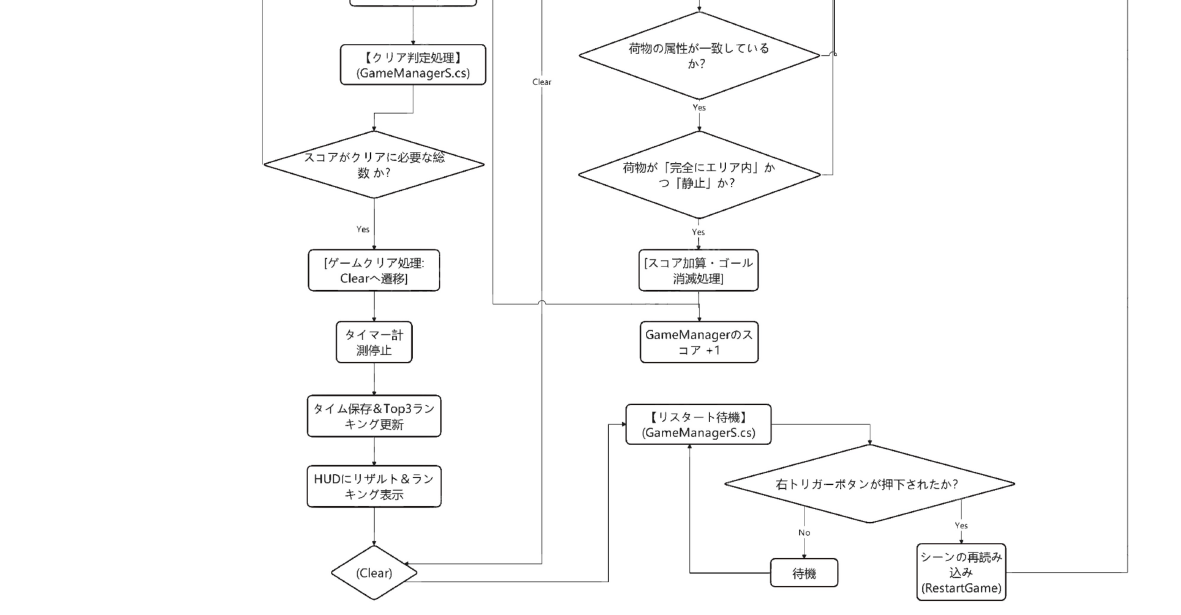
\includegraphics[width=1\linewidth]{images/flow2.png}
    \caption{フローチャート(２枚目)}
    \label{fig:flow2}
\end{figure}
まずユーザの動きはMetaQuest3のHMD本体およびコントローラが検出し，この座標に合わせてロボットの胴体が追従するように処理している．例えば左手の動きの追従であれば，以下に示すスクリプトのように，animatorコンポーネントにおけるIK(Inverse Kinematics)を用いてコントローラの座標から関節角度を算出して上腕と下腕のボーンの動きを決定している．

\begin{lstlisting}
     if (leftController != null)
        {
            animator.SetIKPositionWeight(AvatarIKGoal.LeftHand, 1f);
            animator.SetIKRotationWeight(AvatarIKGoal.LeftHand, 1f);
            animator.SetIKPosition(AvatarIKGoal.LeftHand, leftController.position);
            animator.SetIKRotation(AvatarIKGoal.LeftHand, leftController.rotation);
        }
\end{lstlisting}
コントローラの座標位置は荷物を掴むことができるかどうかの判定にも利用されている．最初に荷物が持ち上げられた瞬間にゲームのループがスタートし，全ての荷物が所定の場所に置かれたと判定されたときに，ループが終了する．荷物がゴールエリアに置かれているかどうかを判定するのは以下のスクリプトで行なっている．正しい荷物がエリア内に入っているかを判定し，荷物が完全に止まったときにゴールの判定をしている．この判定の後，ゴールエリアは自身を非表示にする．
\begin{lstlisting}
     if (cargo != null && cargo.myType == acceptedType)
            {
                if (IsCompletelyInside(cargo.GetComponent<Collider>()) && IsStationary(rb))
                {
                    // 種類も一致し、静止して完全に入った
                    GameManager.Instance.AddScore();
                    rb.isKinematic = true; 
                    cargosInZone.RemoveAt(i);

                    //自分自身（ゴールエリア）を非表示（無効化）にする
                    gameObject.SetActive(false);
                }
            }
\end{lstlisting}
クリア判定が起こったとき，クリアタイムの計測がなされてランキングが表示される．これはHMD内に保存されるものであり，以下のスクリプトで実行されている\begin{lstlisting}
    string resultStr = "";
        for (int i = 0; i < Mathf.Min(3, times.Count); i++)
        {
            PlayerPrefs.SetFloat("Rank" + (i + 1), times[i]);
            resultStr += (i + 1) + "st: " + FormatTime(times[i]) + "\n";
        }
        PlayerPrefs.Save();
\end{lstlisting}
小数点以下３桁までの表示にとどめており，これを保存している．なおクリア後はリスタート待機状態となりコントローラの右トリガーが押下されたときにシーンが再度読み込まれ，初期状態に遷移する．このとき前回およびこれまでのクリア時間のデータは削除されず，以後参照され続ける．


\section{担当作業内容}
\ifdraft
自分が担当した部分について、その作業内容について、箇条書きで記述する。
以下に各担当毎に示す。
\subsubsection{ディレクタ}
\begin{itemize}
    \item グループで1作品を作成する上で、スムーズに作業するためにどのような指示を出したか。また、その結果はどうだったかを述べる。
    \item 作業過程で発生した、グループ作業であるが故の問題やその解決法なども述べること。
    \item ディレクタの他にプログラマまたはモデラを兼任した学生は、そちらの作業内容に力を入れて述べること。ただし、レポートの枚数制限は設けていないのでディレクタの担当作業も書くべき内容があるのであれば、詳細に述べて良い。
    \item ディレクタ専任の学生は、自分の作業を詳細に述べること。
\end{itemize}

\subsubsection{プログラマ}
\begin{itemize}
    \item 作品を動かすスクリプトについて、どの部分を自分が担当したかを述べる。
    \item 作品全体を通しての作業だけで無く、更に具体的にかつ詳細に、共同作業を行った他の担当と、どのような共同作業をしたのかを述べること。
    \item 参考としたスクリプト（基本事例や動作事例など）があればそのスクリプトも挙げ、どの部分をどのように変更したかを述べる。作業を進める上で発生した問題やその解決法、工夫した点を詳細に述べ、その結果どうなったかも説明する。
    \item 作成したスクリプトは本章の最後に名称と機能をまとめた一覧を設けること。その際、引用したスクリプトを改変した場合には、引用元を明示すること。
\end{itemize}


\subsubsection{モデラ}
\begin{itemize}
    \item 作品内に表示させたCGオブジェクトのどの部分を自分が作成したのかを説明する。作品全体を通しての作業だけで無く、更に具体的にかつ詳細に、共同作業を行った他の担当と、どのような共同作業をしたのかを述べること。
    \item モデル作成の過程において発生した問題やその解決法を述べる他、モデルを完成させるために工夫した点などを述べる。
    \item 完成したオブジェクトの外観図の他、ワイヤーフレーム図、描画ポリゴン数なども記載し、オブジェクトがどのような構造になっているかを詳しく説明する。
    \item テクスチャを使用しているならばそのテクスチャの画像も提示する。Webなど、自分の作品でないテクスチャに関しては図と共にその出典も必ず記載すること。
    \item オブジェクトを作成するにあたり、何らかのモデルを参考にした場合（キャラクターなど）、参考したモデルの画像の提示及び出典を記載する。
\end{itemize}
\fi
% 以下に本文を書く
私の役割はプレイヤーが操作するロボットのモデリングであった．作成したモデルを図\ref{fig:robot_center},\ref{fig:robot_side},\ref{fig:robot_top}に示す．このモデルがプレイヤーの持つコントローラやHMDの動きとリンクしてアニメーションが行われるように，UnityのHumanoid型に適合するアーマチュア構造を取り入れた\cite{weight}．そのためにロボットのモデルもその型に適合するように，腕のパーツは上腕，肘，下腕，手をそれぞれ作成し，脚のパーツについても上脚，膝，下脚，足をそれぞれ作成した．

\begin{figure}[htbp]
    \centering
    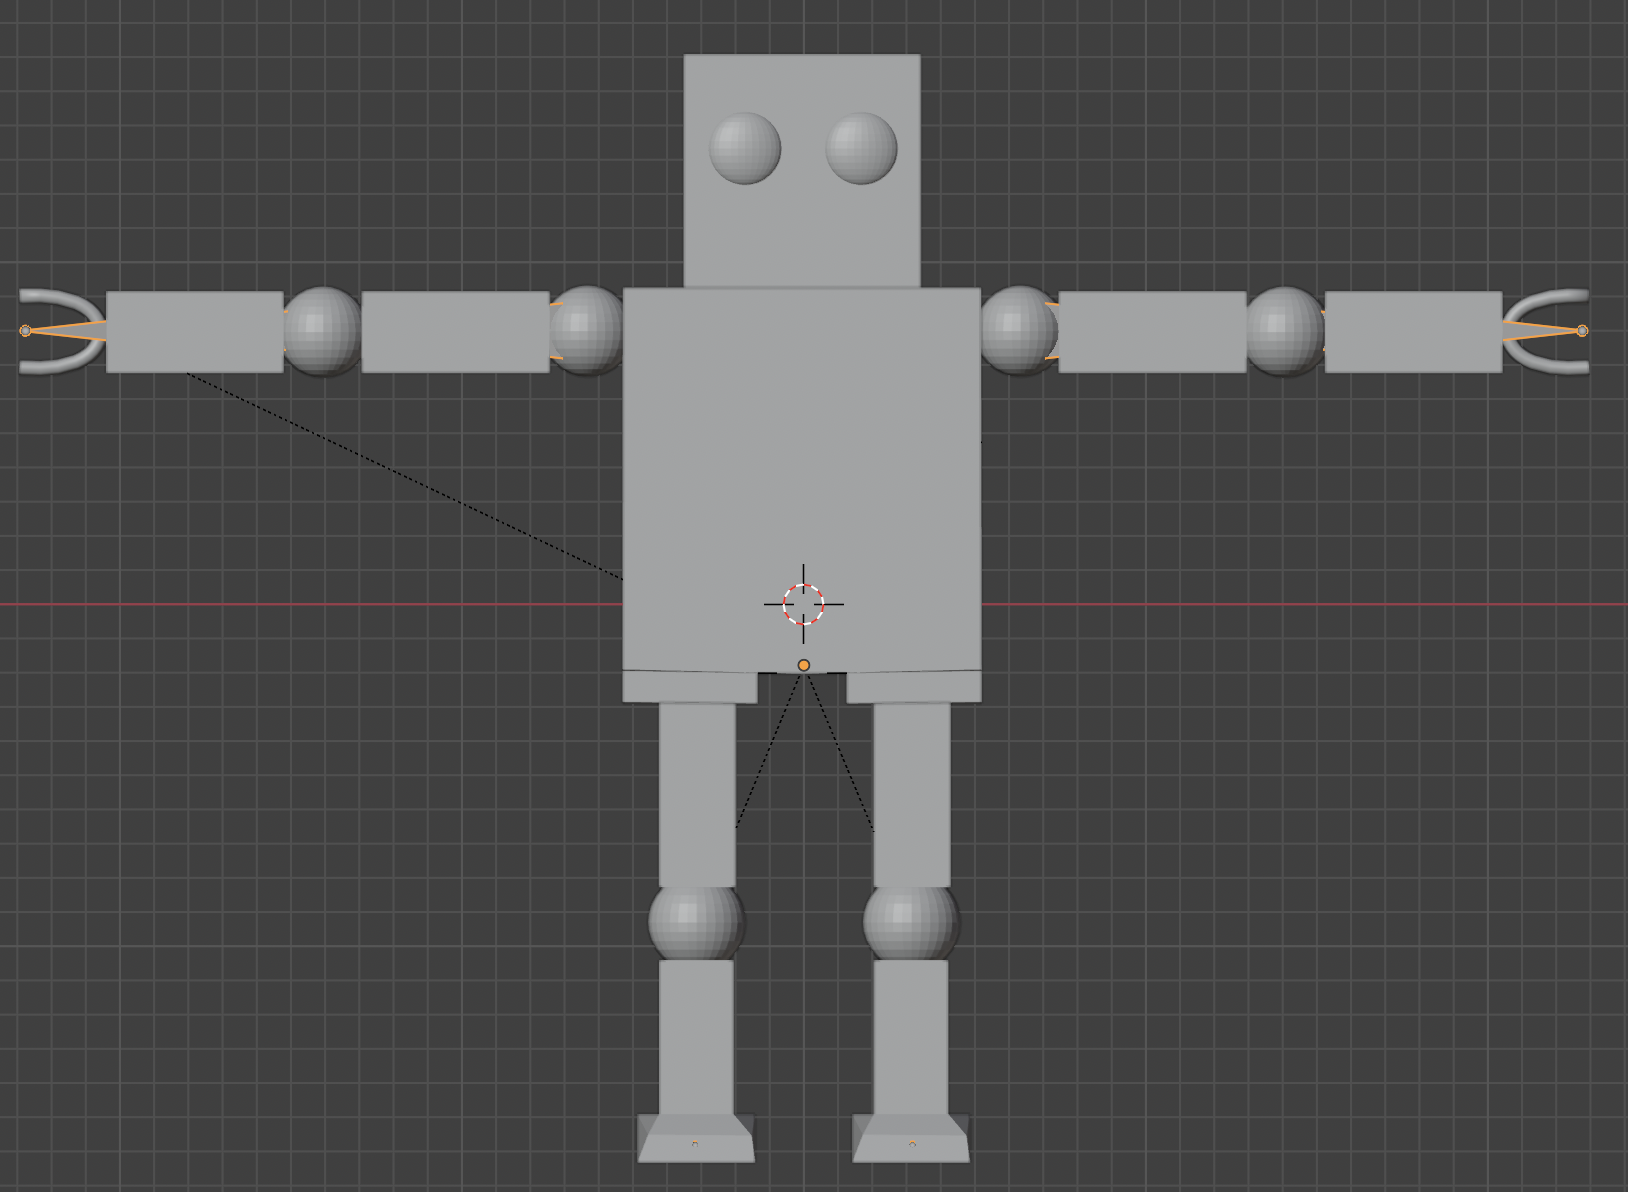
\includegraphics[width=0.6\linewidth]{images/model/robot_center.png}
    \caption{正面から見たモデル}
    \label{fig:robot_center}
\end{figure}

\begin{figure}[htbp]
    \centering
    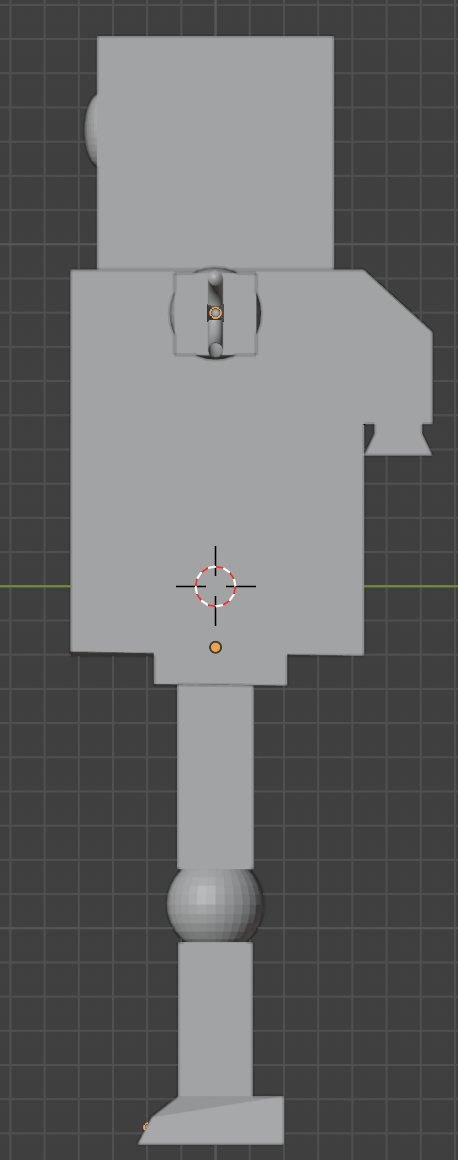
\includegraphics[width=0.3\linewidth]{images/model/robot_side.png}
    \caption{側面から見たモデル}
    \label{fig:robot_side}
\end{figure}

\begin{figure}[htbp]
    \centering
    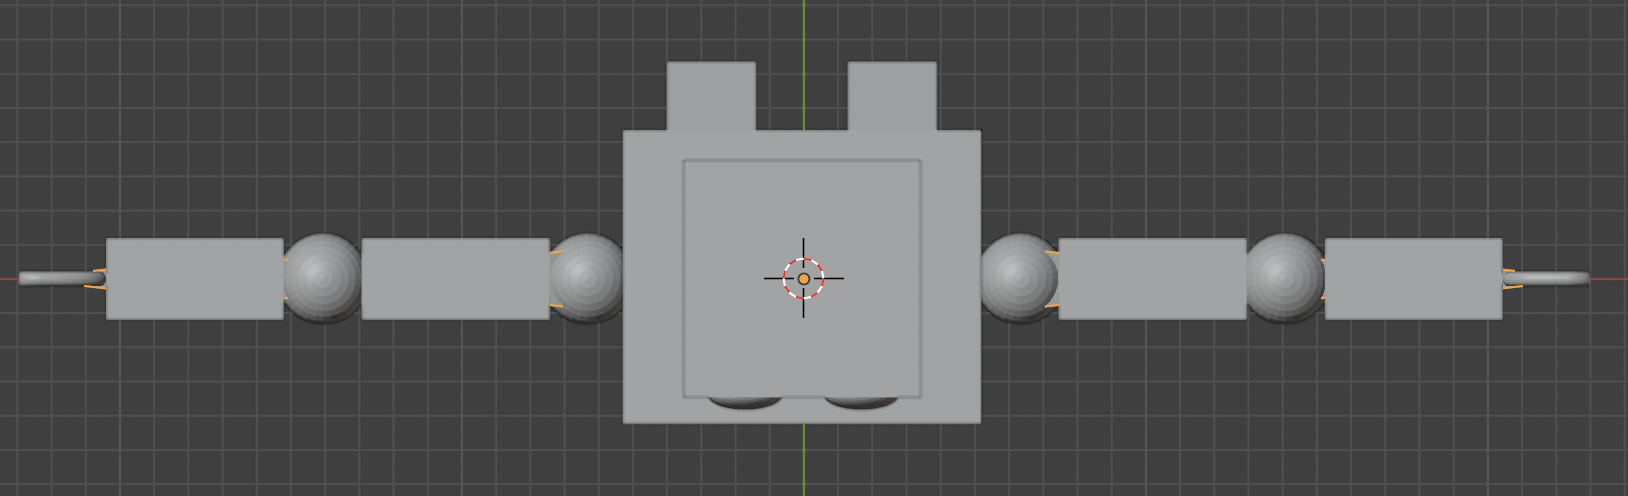
\includegraphics[width=0.7\linewidth]{images/model/robot_top.png}
    \caption{上から見たモデル}
    \label{fig:robot_top}
\end{figure}

次に\cite{weight},\cite{riging}を参考にして作成した，ロボットのアーマチュア構造を図\ref{fig:robot_bone}に示す.アーマチュアを形成するオブジェクトの末端である「ヘッド」や「テール」と呼ばれる部分を，動かしたいパーツの位置にそれぞれ合わせることで，モデルが意図した動きをするように気をつけた．ここで，アーマチュアと3Dモデルのパーツに親子関係を設定し，blenderをポーズモードにて下腕のボーンの動作を確かめた．この時の結果は図\ref{fig:fail_2}に示すように，左の下腕を上方向に動かしたにもかかわらず，右の下腕が下方向に移動している．これは図\ref{fig:weight_before}に示すように，本来であれば左腕のみに追従させるべき"UpperArm L"と"LowerArm L"のボーンが右腕の動きに割り振られているからである．このような動作の不一致が多くのパーツで発生した．

\begin{figure}
    \centering
    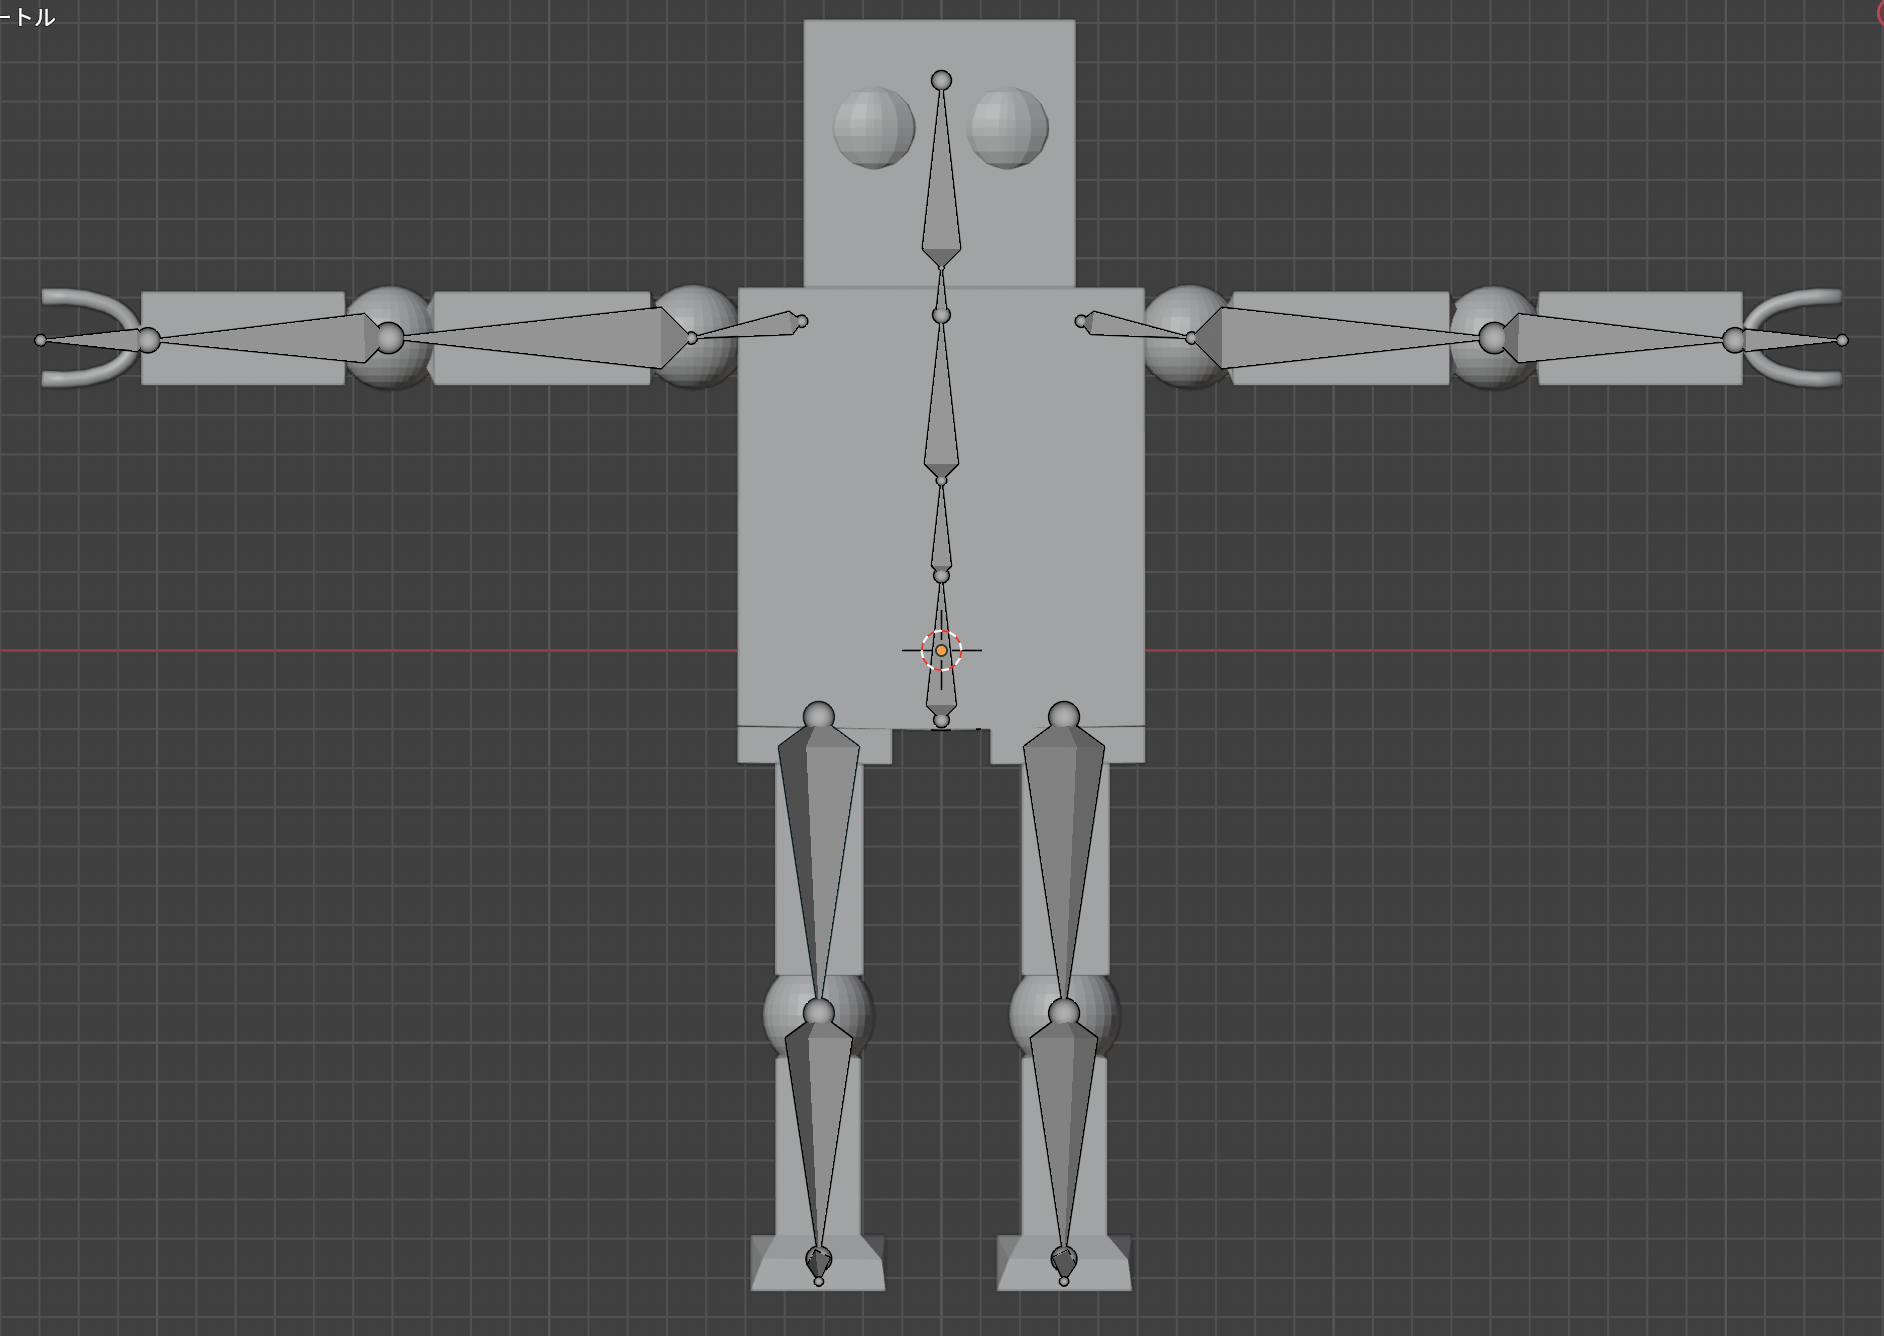
\includegraphics[width=0.7\linewidth]{images/model/アーマチュア.png}
    \caption{ロボットのアーマチュア構造}
    \label{fig:robot_bone}
\end{figure}

\begin{figure}
    \centering
    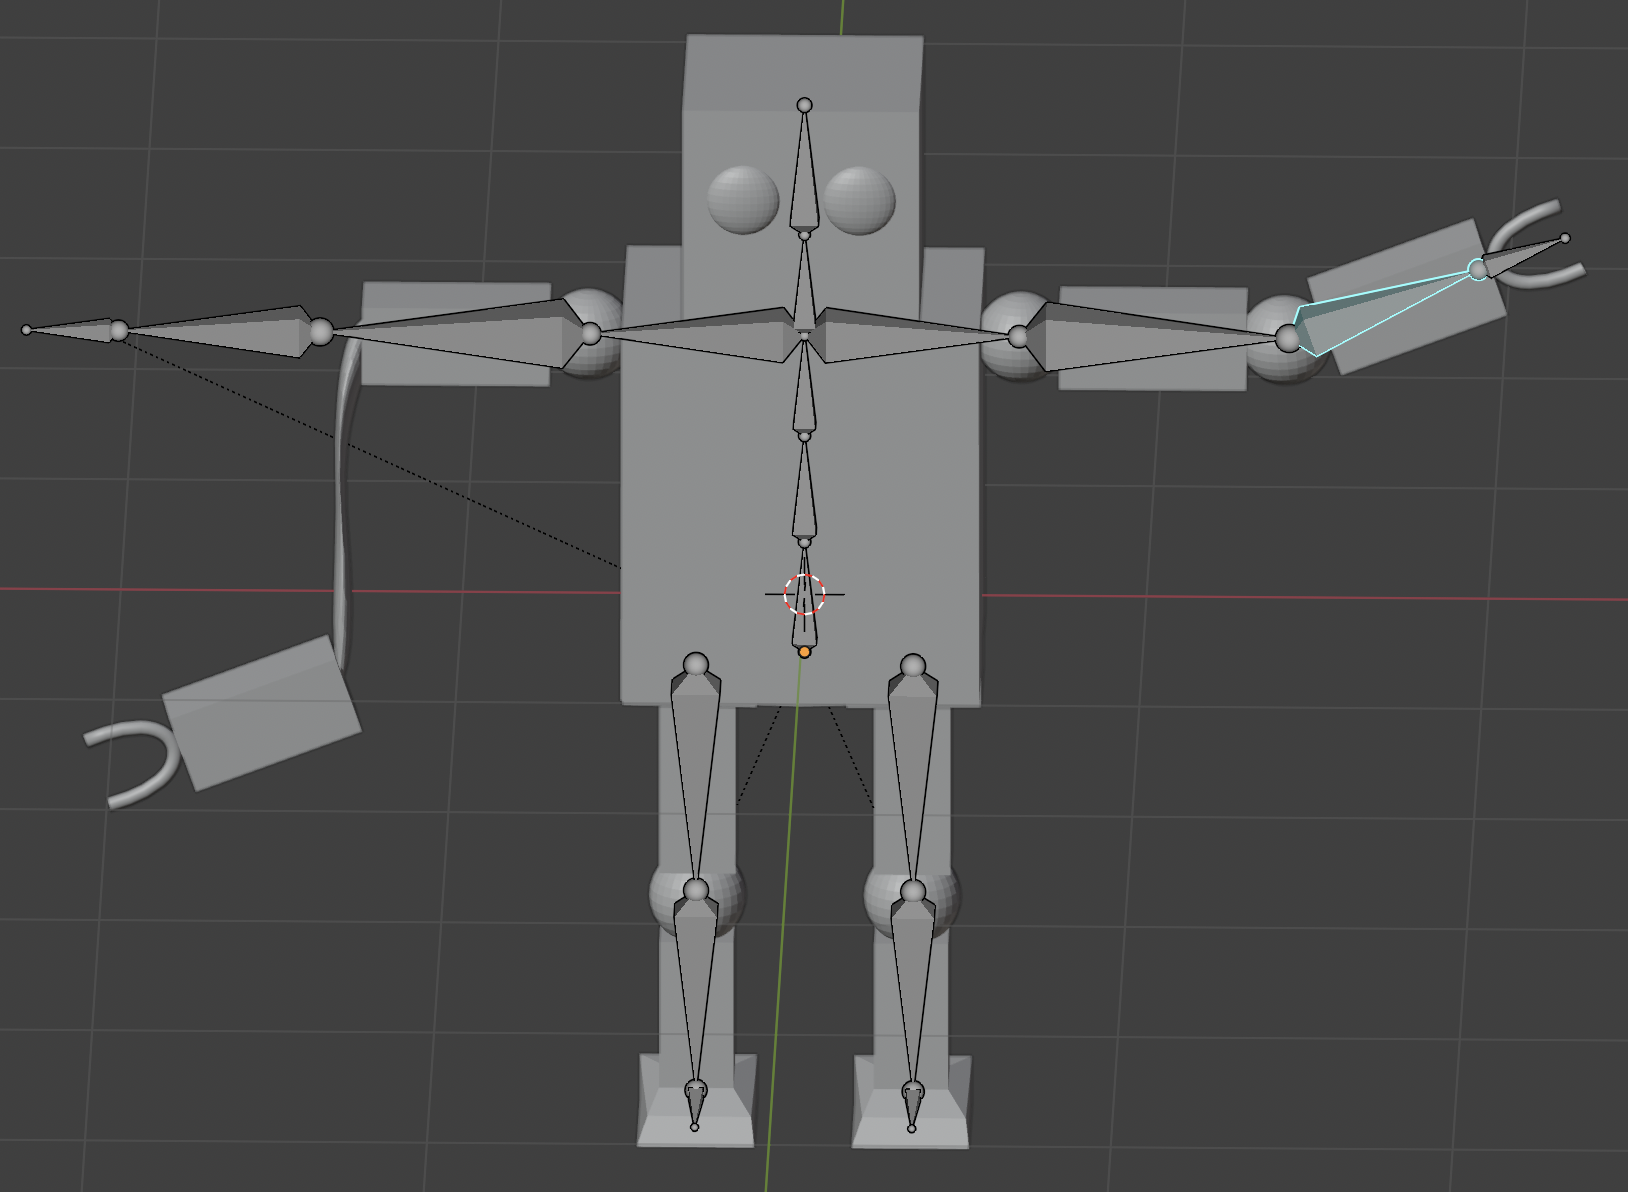
\includegraphics[width=0.7\linewidth]{images/model/fail_2.png}
    \caption{ウェイトの設定が失敗した時の例}
    \label{fig:fail_2}
\end{figure}

\begin{figure}
    \centering
    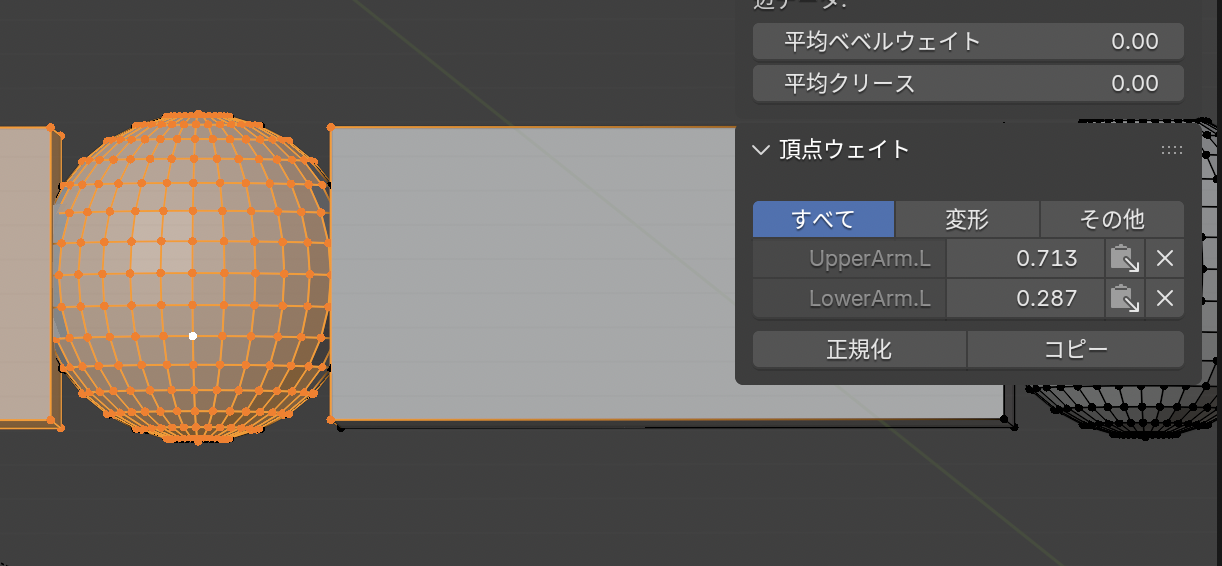
\includegraphics[width=0.7\linewidth]{images/model/weight_before.png}
    \caption{ウェイト設定前}
    \label{fig:weight_before}
\end{figure}

そこでこの問題を解消するために，モデルの全ての頂点に対して，それぞれがどのボーンに追従するかを設定した．先ほどの右の下腕を編集した結果を図\ref{fig:weight_after}に示す．想定通りに動くように，右腕を"UpperArm R"と"LowerArm R"に追従するように割り振った．このような設定を行い，再度ボーンの動作を確かめた結果を図\ref{fig:weight_success}に示す．右腕のみならず，全てのボーンにその位置にある3Dモデルのパーツが追従していることがわかる．このような動きの設定によって，前述のUnity上でのHumanoid型のアニメーションを適用することができ，歩行時のアニメーションなどをスムーズに実装することに貢献した．

\begin{figure}
    \centering
    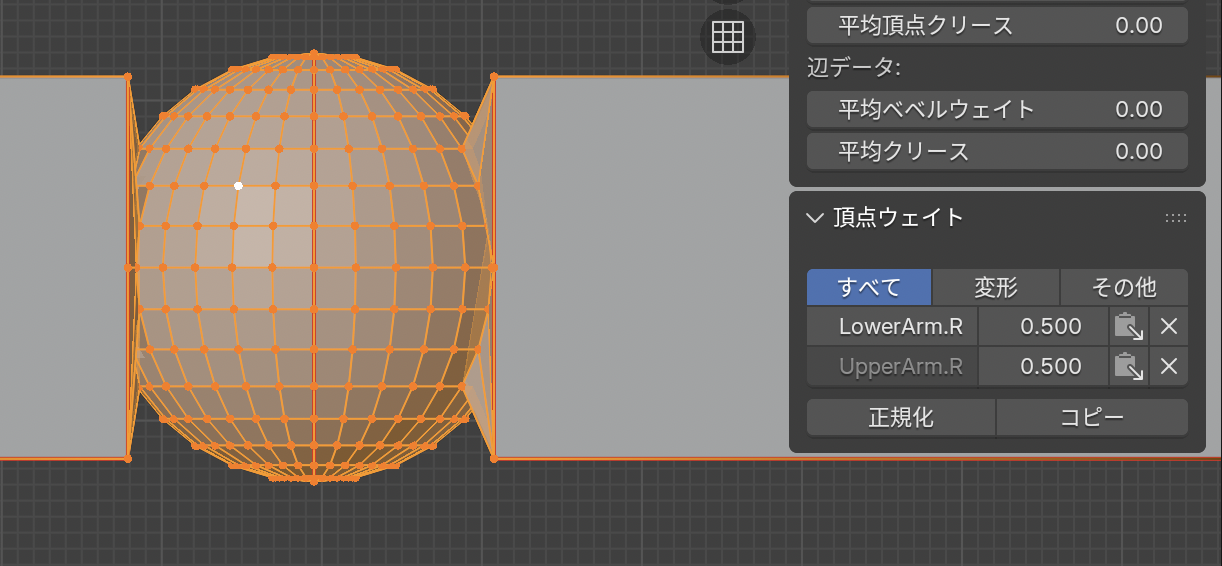
\includegraphics[width=0.75\linewidth]{images/model/weight_after.png}
    \caption{ウェイト設定後}
    \label{fig:weight_after}
\end{figure}

\begin{figure}
    \centering
    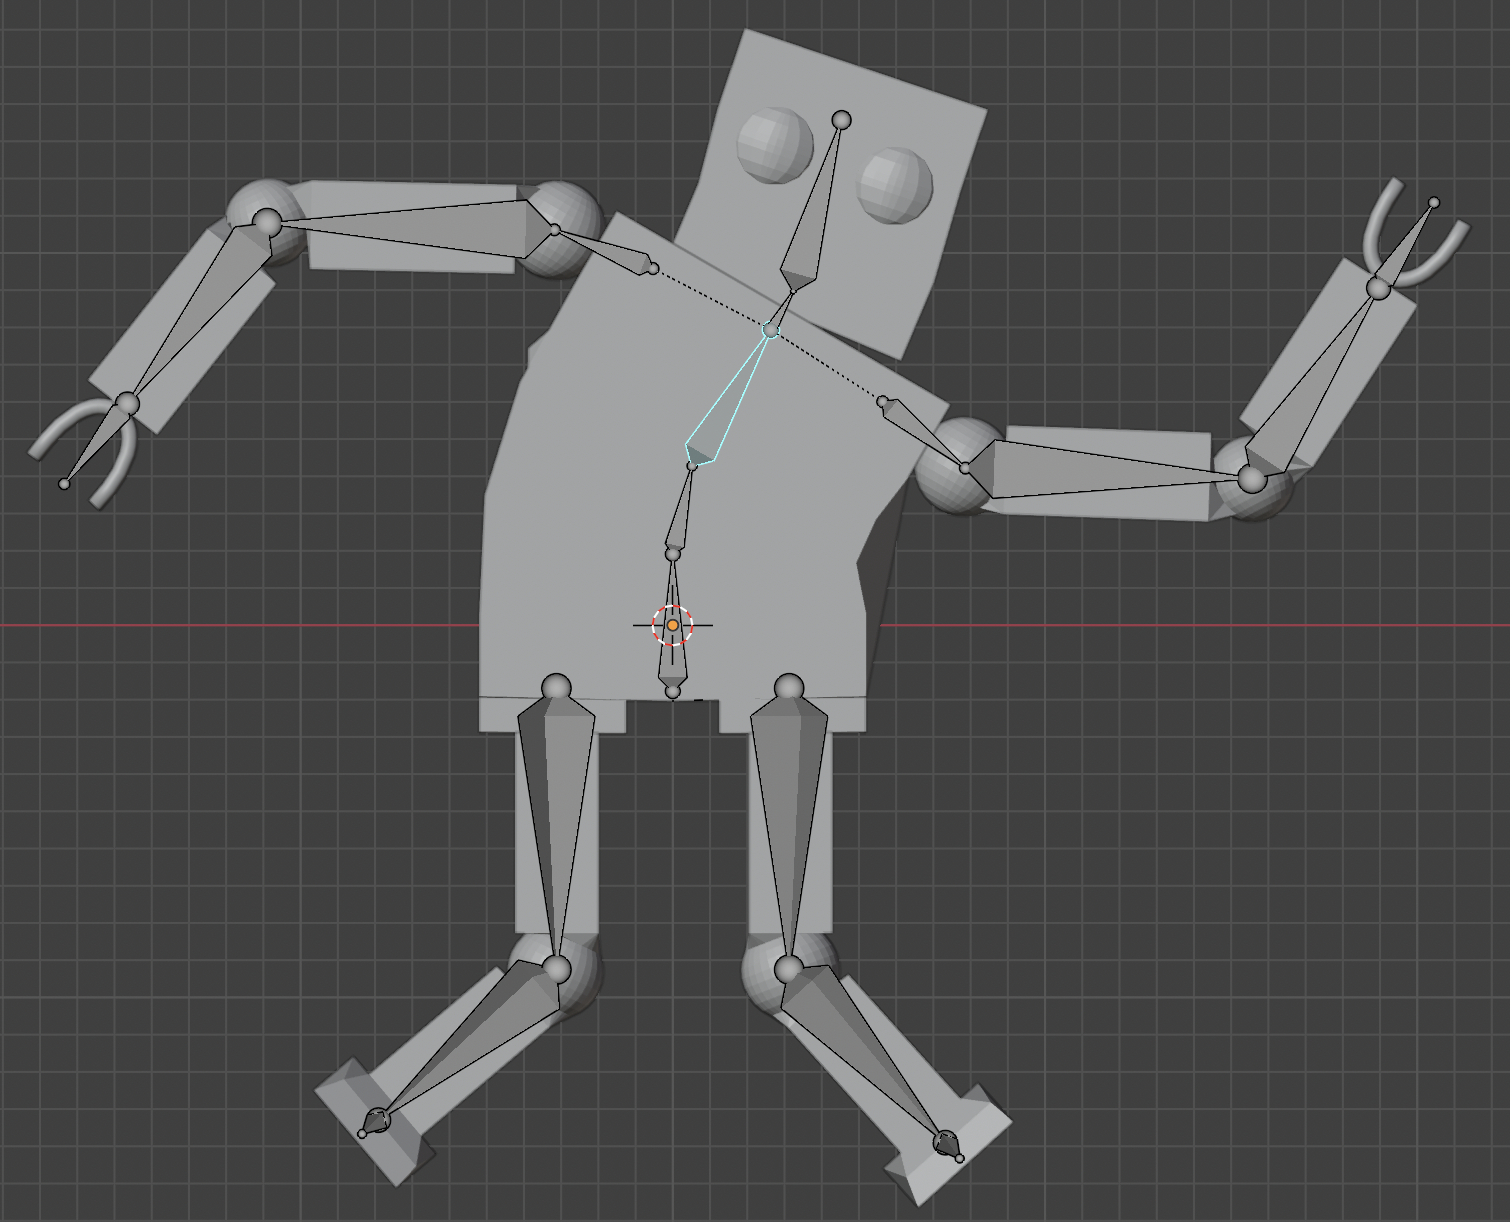
\includegraphics[width=0.75\linewidth]{images/model/weight_success.png}
    \caption{ウェイトの設定が成功した時の例}
    \label{fig:weight_success}
\end{figure}

完成したモデルのワイヤーフレーム図を図\ref{fig:robot_flame}として示す．ただしこの図では，ロボット本体のモデルの構造を見やすくするために，ボーンの構造は不可視化している．ロボットのパーツは，頭部・胴体・右腕・左腕・右脚・左脚の6パーツに分かれており，それぞれのパーツを構成する頂点は他のパーツとは繋がっていない．頂点数は4,930であり，これはデスクトッププラットフォームにおける理想的な範囲とされる4,000個\cite{porigon}を超えてしまった．この原因としては，特に膝関節部分において滑らかな変形を実現できるようにポリゴン数を増やしすぎてしまったことであると考えられる．

\begin{figure}
    \centering
    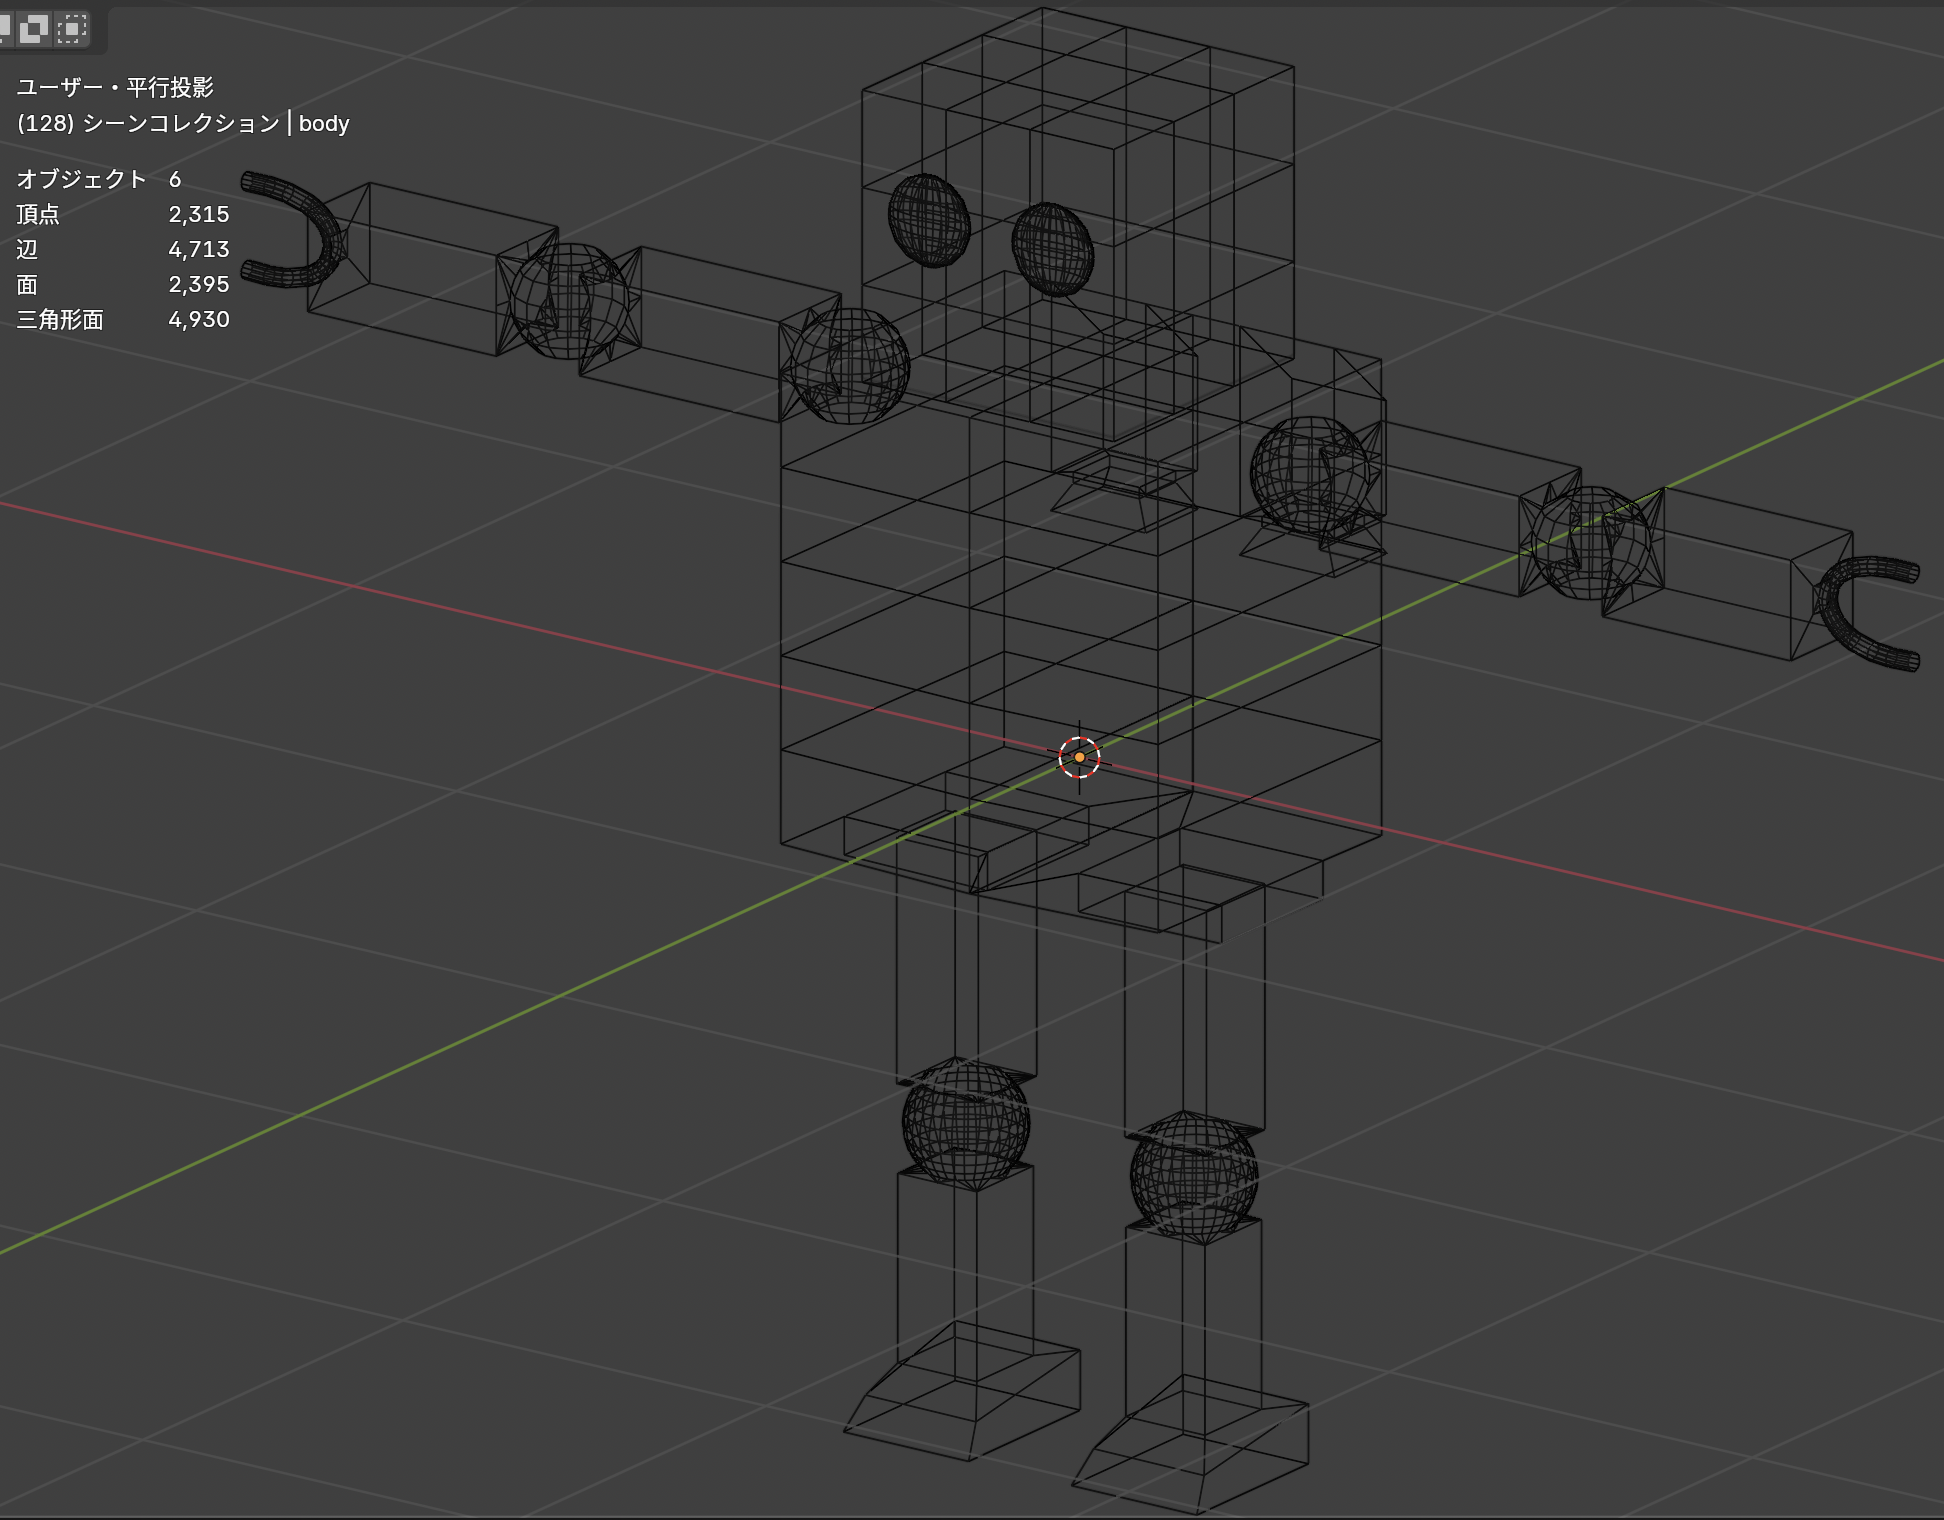
\includegraphics[width=0.75\linewidth]{images/model/robot_flame.png}
    \caption{Caption}
    \label{fig:robot_flame}
\end{figure}
次に作成したテクスチャを図\ref{fig:head},\ref{fig:body},\ref{fig:arm},\ref{fig:leg}で示す．これらのテクスチャ画像は図\ref{fig:uv}のようにUV展開を行い，その上からテクスチャペイント機能により色を塗ることで作成した．UV展開後にどの面がどの部分の展開であるのかが分かりやすい展開図を得るために，展開する時の切れ目となる辺をうまく選択する必要があった．

\begin{figure}
    \centering
    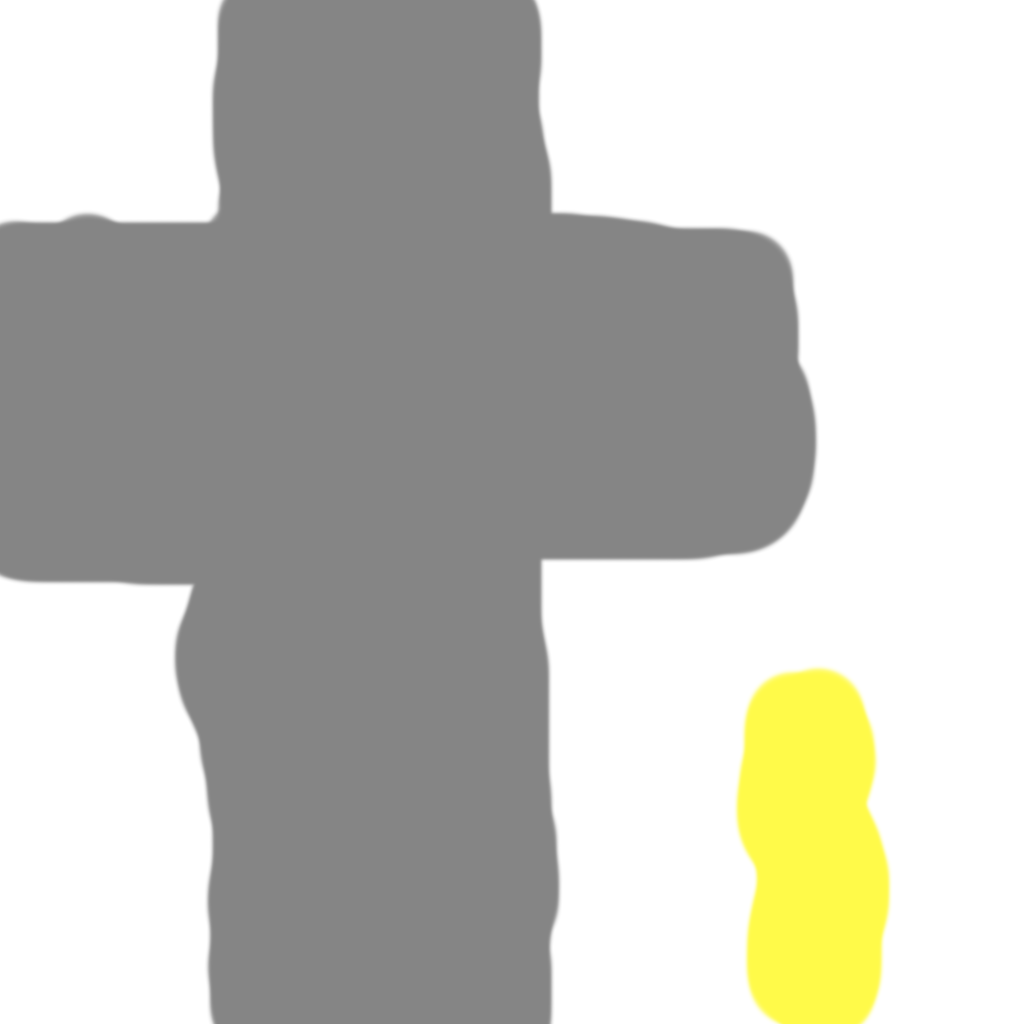
\includegraphics[width=0.5\linewidth]{images/model/head.png}
    \caption{頭のテクスチャ画像}
    \label{fig:head}
\end{figure}

\begin{figure}
    \centering
    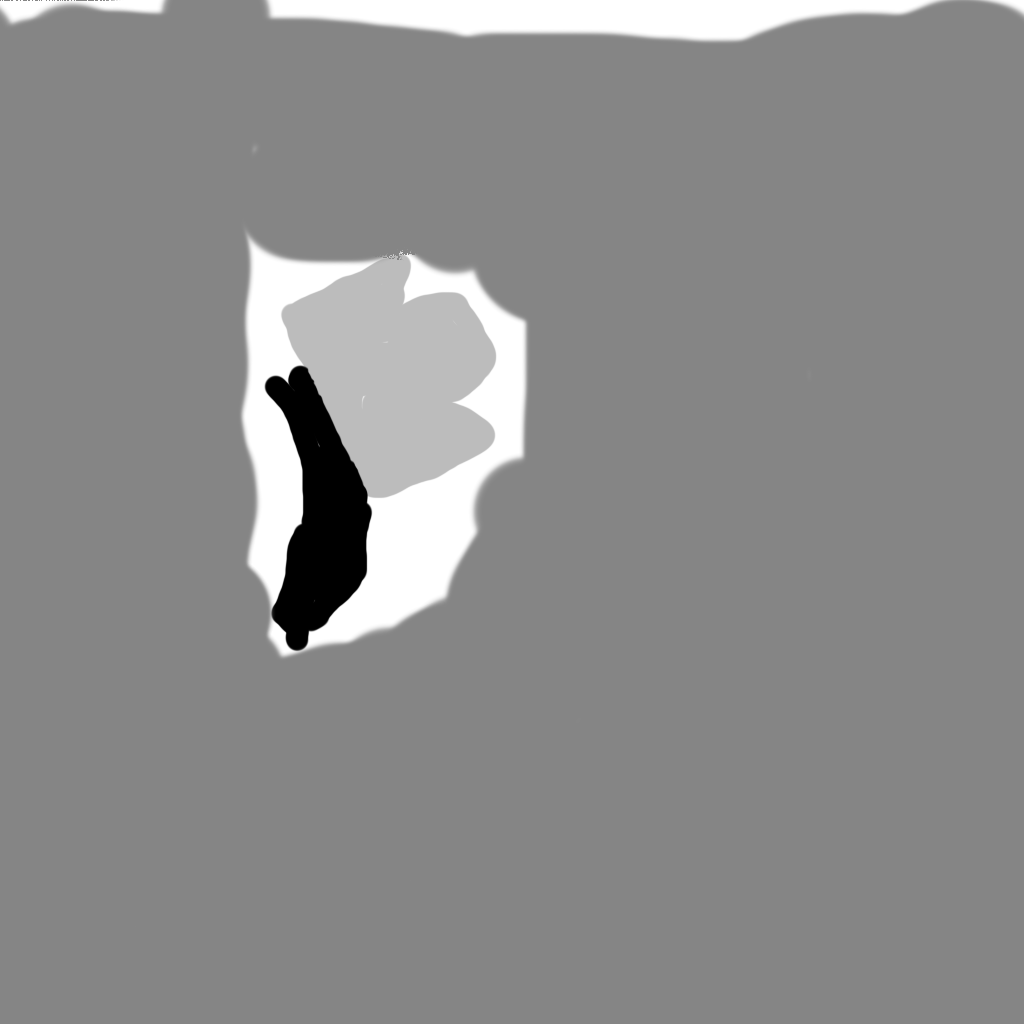
\includegraphics[width=0.5\linewidth]{images/model/body.png}
    \caption{胴体のテクスチャ画像}
    \label{fig:body}
\end{figure}

\begin{figure}
    \centering
    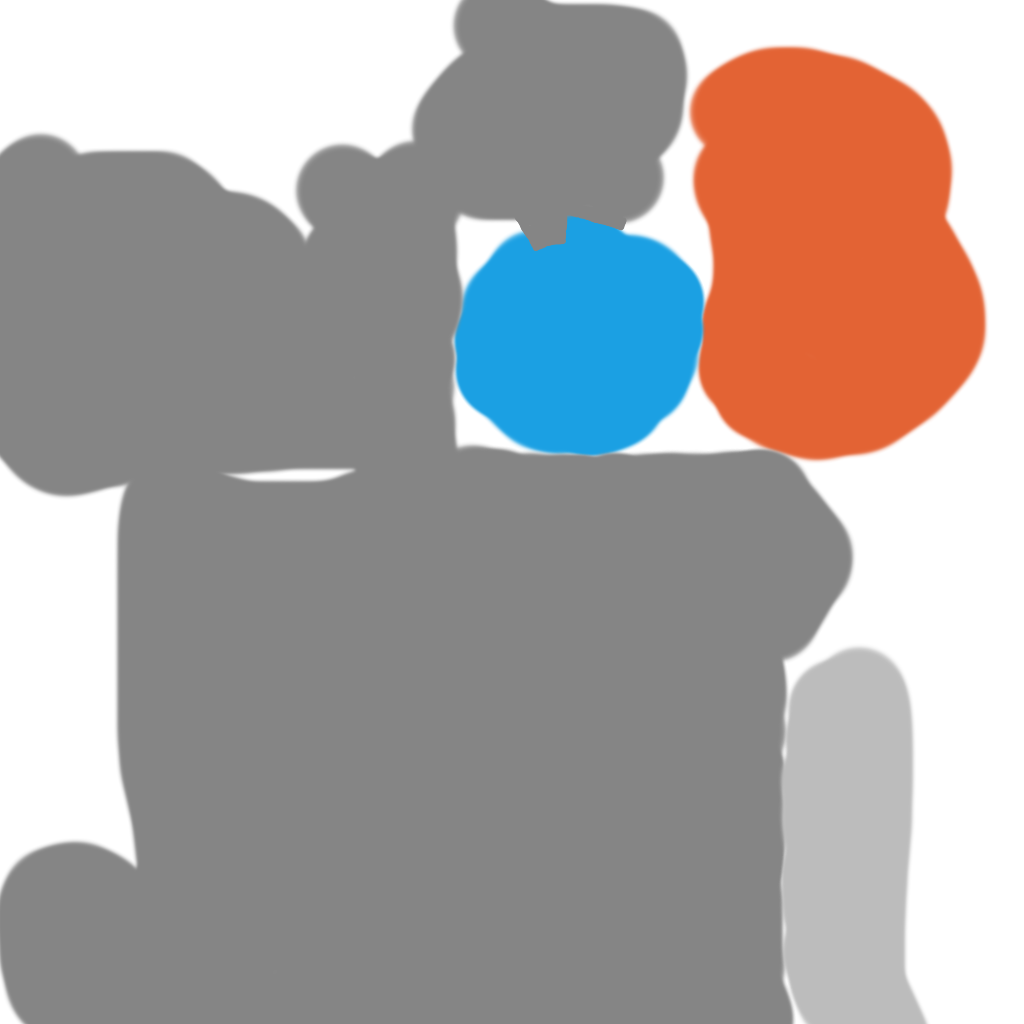
\includegraphics[width=0.5\linewidth]{images/model/armR.png}
    \caption{腕のテクスチャ画像}
    \label{fig:arm}
\end{figure}

\begin{figure}
    \centering
    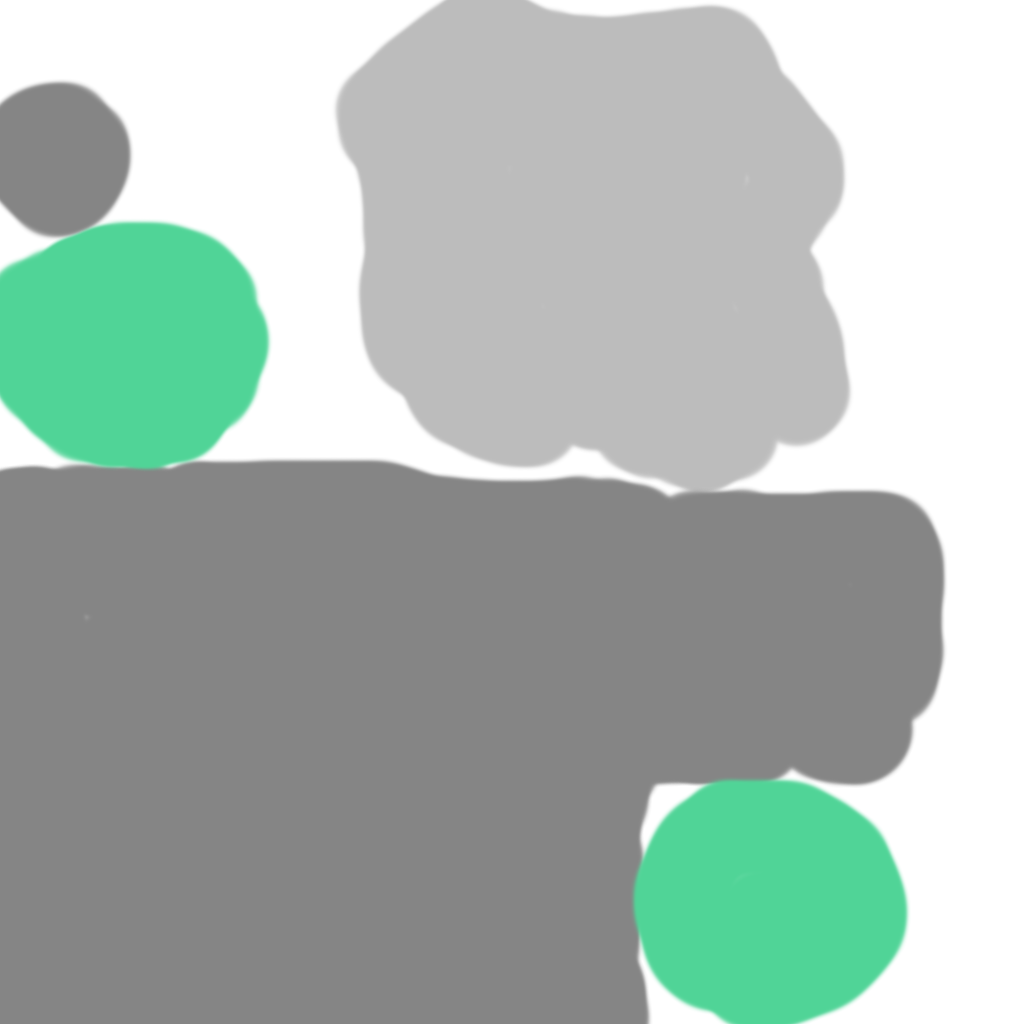
\includegraphics[width=0.5\linewidth]{images/model/LegR.png}
    \caption{脚のテクスチャ画像}
    \label{fig:leg}
\end{figure}

\begin{figure}
    \centering
    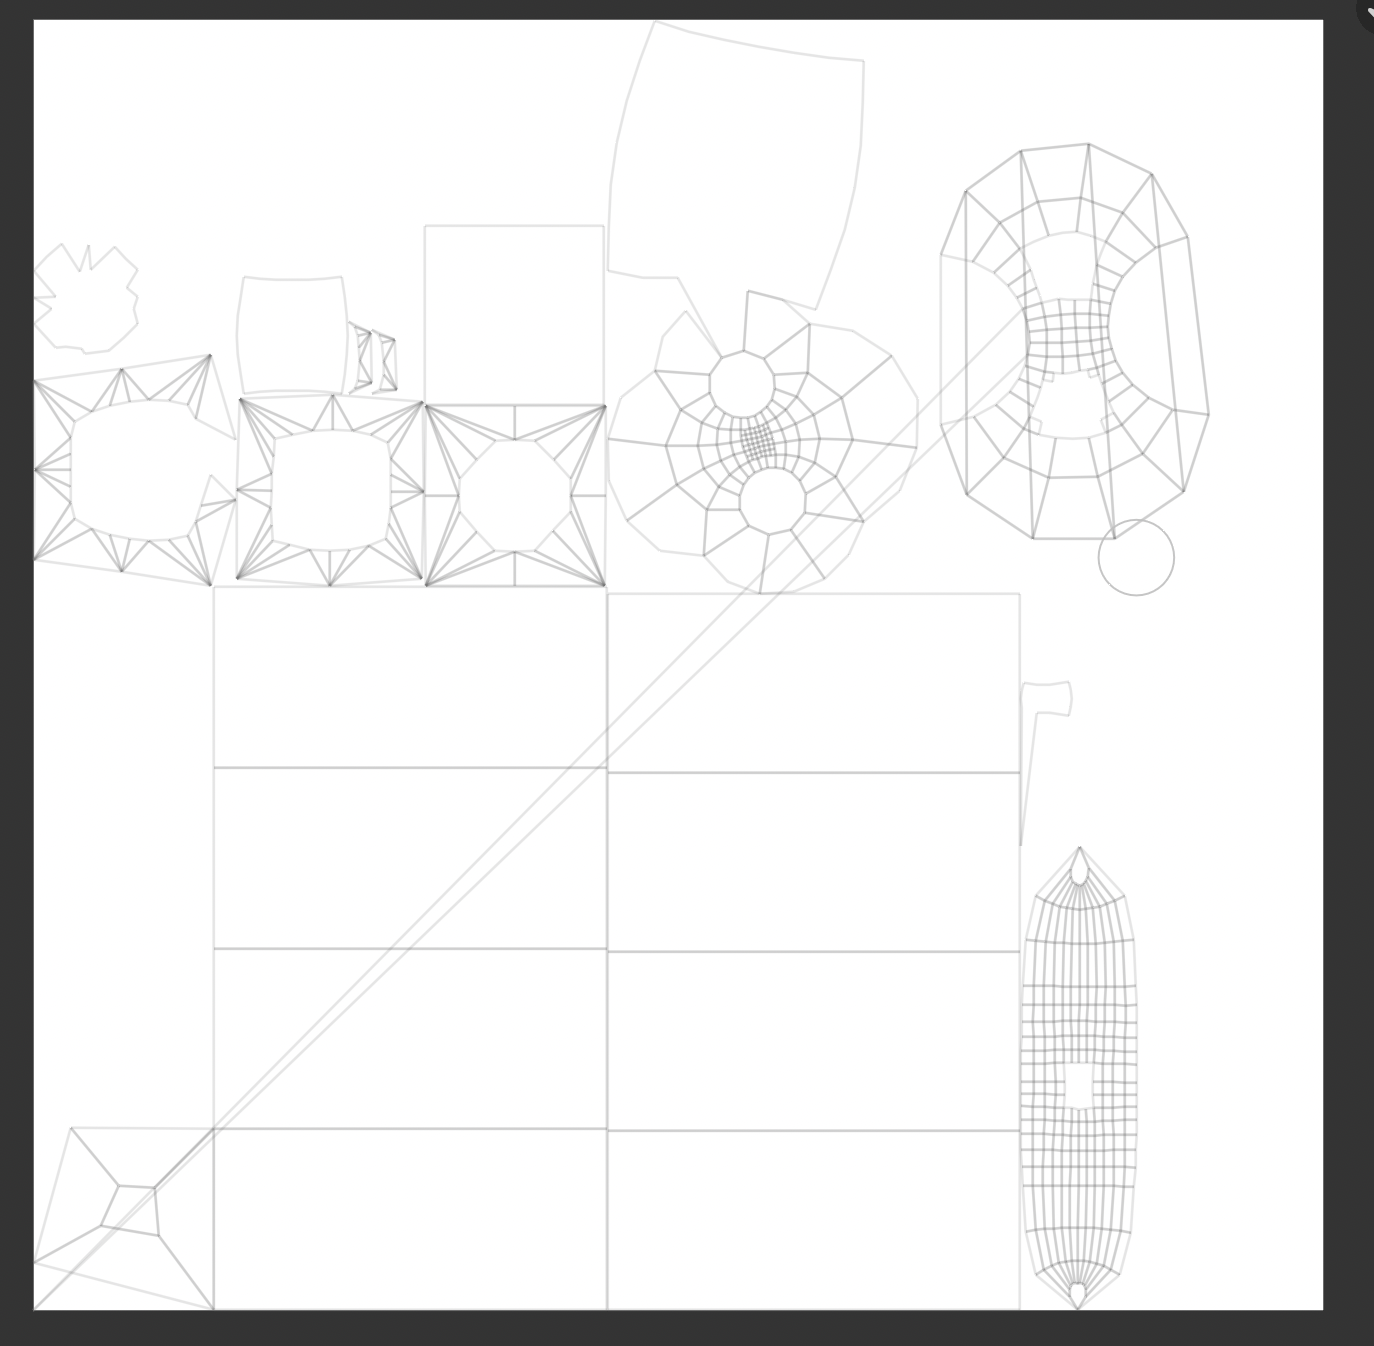
\includegraphics[width=0.5\linewidth]{images/model/UV.png}
    \caption{UV展開の後テクスチャペイントをする}
    \label{fig:uv}
\end{figure}

これらのテクスチャを適用したモデルの画像を図\ref{fig:render}
に示す．意図した通りの位置に色がついていることを確認できる．
\begin{figure}
    \centering
    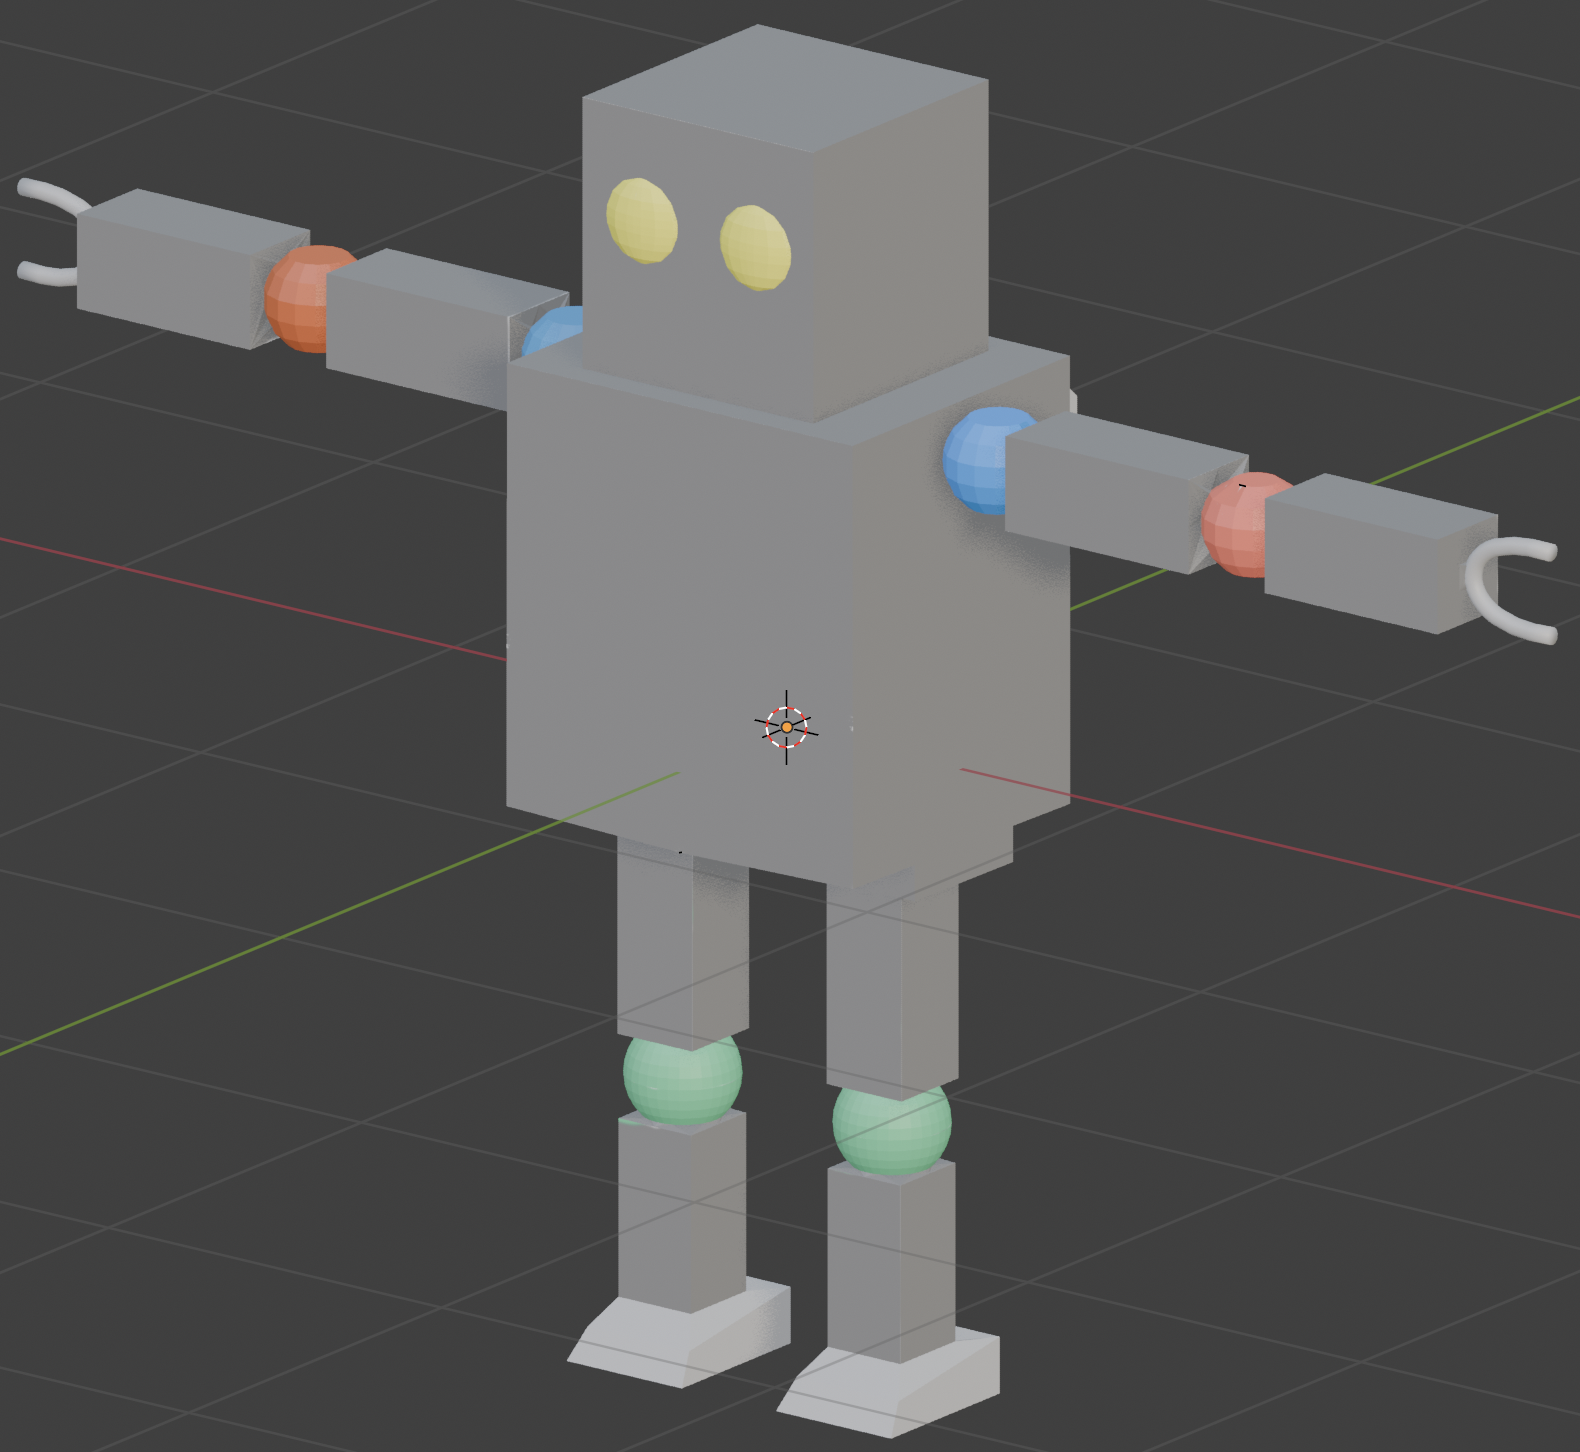
\includegraphics[width=0.75\linewidth]{images/model/robot_render.png}
    \caption{テクスチャを適用したモデルの画像}
    \label{fig:render}
\end{figure}

\section{VR実験に関する考察}
\ifdraft
課題作品を構築する過程で得られた知見について、客観的に述べる。

前半の個人実習ではVRシステムにおけるシミュレーション機能の重要性について論ずる。
後半のグループ共同制作では、3章で述べた開発計画を100\%として、自己判断で何\%の完成度となったかをまず記述し、その判断の理由を、予定を上回る成果、あるいは逆に、計画を立てたが実装できなかった機能、表示できなかったオブジェクトに関して具体的に記し、その原因を分析すること。ここで考慮すべき原因とは授業の時間制限ではなく、技術的制限（実行環境、インタラクションデバイス等）である。さらに自らの工夫で達成できた点で、特に記しておきたい技術的分析があればここに記述する。

いずれも、個人の実験の感想である``良かった''、``楽しかった''ではなく、工学実験の結果に対して、客観的に記述することを心がけること。
\fi
% 以下に本文を書く
前半の個人実習においては，VRシステムにおけるシミュレーション機能の重要性を学んだ．使用するシミュレーション環境によって結果に誤差が生まれることや，没入感を与えるVRシステムの実現には，人間が知覚して違和感のないような現実世界と同様の物理環境を整える必要がある．そのため，その誤差が実装する機能の動作に影響のない範囲にとどまるかどうかを検証する必要があるように思われた．逆にこのシミュレーション精度を人間が知覚できる境界付近まであえて粗くする事によって，自然な体験を与えられるシステムをコンピュータのリソースを大きく割く必要なく実装可能であると考えた．

後半のグループ共同制作での完成度は80\%である．その理由は第3章，4章で述べた作品制作の構想と最低限実装すべき機能のほとんどを実現することができたからである．特に第4章で述べた作品における課題は全てクリアすることができ，VRシステムとして成立する挙動を実現することができた．一方で残る課題は，第3章で述べた作品のコンセプトを十分に反映させた作品に仕上がらなかったからである．今回の制作において，ユーザは掴んだ荷物を投げ飛ばすことができ，かつ荷物をどれだけ雑に扱ったとしても所定の位置にさえおけばゲームクリアとなる．しかしこの作品のテーマは倉庫における荷物整理作業をロボットの操作によって行うものであり，現実ではたとえ低重力下であっても，荷物を雑に扱えば損傷する可能性が高い．この作業をVRシステム上でよりリアリティを持って体験するためには，荷物に耐久ゲージをつけるなどして，丁寧に配置させるようにするための仕組みが必要であったと考えられる．


\section{結論}
\ifdraft
1章で実験を受講するにあたっての自分の目的と課題とした部分について、実験全体を通して評価を行う章である。目的と課題について、個人実習、グループ制作を通してどのような学びがあり、その課題、目的がどの程度達成できたのかを評価する。

また、主観的に、本実験を通して感じたことを記述してよい。ただし、単に面白かったとか、運営上の不備に関する不満を書くのではなく、この実験から何を学んだのか、何を感じたのか、学生としての見識ある感想・抱負等を期待する。
\fi
% 以下に本文を書く
第1章において私が目的と課題としたのは，VRシステムの制作にあたって必要なシミュレーション技術とインターフェース技術について理解しこれらを使えるようになることである．シミュレーション技術の理解と習得については，まず個人実習においてthree.js環境とUnity環境でのシミュレーション結果と解析解とを比較する事によって，これらの環境の差について学ことができ，これらの特性をどのようにVRシステムのシミュレーションに活用することができるのかを学ぶことができた．またインターフェース技術については，私は作品制作においてモデラとしての役割の中で，3Dモデルをユーザの頭や腕の動きにリンクさせて動かすための方法を学んだ．MetaQuestからの動きの入力をUnity上で3Dモデルに反映させるのは，用意されたアセットによって思っていたよりも容易に実装することができたが，そもそもの3Dモデルの制作過程の中で，ボーンを設定したときに意図した通りの動きをさせるのに苦労した．しかし参考文献として提示したwebページから学んだ方法を駆使しつつ，人体モデルの大まかな動きの作り方を習得することができたと感じている．

今後の展望としては，まず今回の制作ではあまり関わらなかった作品制作過程でのUnity上のシミュレーション周りのプログラミングについての見識を深めたいと考えている．モデルの制作に関わる技術は最低限得られたため，次は自身がVR機器との連携部分についてのインタラクション機能を理解して実装できるような技術を身につけたいと思う．またモデルの制作についても，今後はより品質の高いモデルを制作できるようになり，またその分だけモデルのポリゴン数は増えると思うが，そのようなモデルでも違和感のないアニメーションを実現できるボーンに対する動きのウエイト付けができるように学びを深めたいと感じた．

またVR実験最終日の発表とデモ体験会では，他のグループの作品を体験し，また自身のグループの作品を体験してもらうことでお互いに評価し合う事になり大変勉強になった．良い感想をもらうこともあれば改善点のフィードバックをもらうこともあり，お互いに学び合う環境があったことは非常にためになった．

\ifdraft
\section{参考文献について}
参考にした文献、インターネット上の情報などを参考文献として記載する。全ての参考文献は本文からかならず引用されていなくてはならない（参考になった文献リストではない）。記載の際には記述のフォーマットは\href{http://jipsti.jst.go.jp/sist/perusal/}{科学技術情報流通技術基準（SIST）}で紹介されるフォーマットを参考にすること。BiBTeXを用いて記述しても良い（むしろ推奨する）。

\section{おまけ}
数式は式\ref{eq:energy}のように書く。
\begin{equation} \label{eq:energy}
  E=mc^{2}
\end{equation}

本文中で文字列をそのまま表記したい場合は\verb|ball_velocity.y|のように文字列をくくる。

図を挿入したい場合は\verb|images|フォルダに図のファイルを入れた上で以下のように書くと図\ref{fig:example}のように参照できる。図のキャプションは\verb|figure|環境の中で\verb|\caption{フロー図}|のように書く。

\begin{figure}[htb]
    \centering
    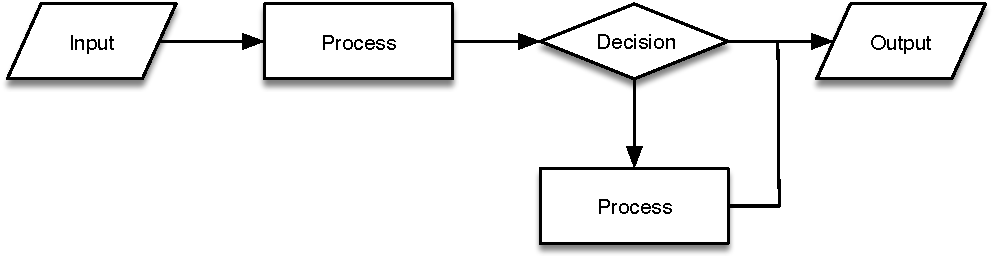
\includegraphics[width=0.7\linewidth]{images/flow.pdf}
    \caption{フロー図}
    \label{fig:example}
\end{figure}

プログラムのソースコードはリスト\ref{lst:example}のように書ける。
 \begin{lstlisting}[caption=ソースコード（JavaScript）の抜粋,label=lst:example]
   if(ball.position.y < 0.5 ) {
     ball_velocity.y = 0.0;
   }
 \end{lstlisting}
\fi

% 参考文献はbibtexで
\bibliography{references}
\bibliographystyle{plain}





\end{document}




% \begin{figure}[htbp]
% \centering
% \includegraphics[scale=0.2]{images/lena.jpg}
% \caption{A standard test image widely used in the field of image processing.}
% \label{fig:lena}
% \end{figure}


